\documentclass[11pt,a4paper,oneside,openany]{book}
\usepackage{stc-common}
\addbibresource{bibliography.bib}

\hypersetup{
  pdftitle={Sleep-Time Compute를 위한 Training Background},
  pdfauthor={Samsung SAIT Neural Memory Study},
  pdfsubject={Training foundations for sleep-time compute},
  pdfkeywords={training, continual learning, sleep-time compute, memory, LoRA, reinforcement learning}
}

\title{Sleep-Time Compute를 위한\\Training Background}
\author{Samsung SAIT Neural Memory Study}
\date{Source freeze: 2026-08-05\\Build edition: 1.0}

\begin{document}
\hypersetup{pageanchor=false}
\begin{titlepage}
  \centering
  \vspace*{20mm}
  {\sffamily\bfseries\color{STCNavy}\fontsize{28}{34}\selectfont
   Sleep-Time Compute를 위한\par Training Background\par}
  \vspace{8mm}
  {\Large 학습을 처음 접하는 시스템·메모리 연구자를 위한 독립 참고서\par}
  \vspace{18mm}
  \begin{tcolorbox}[width=0.84\textwidth,colback=STCMist,colframe=STCBlue,boxrule=0.8pt,arc=2mm]
  이 책은 ``용어 사전''이 아니라, 데이터가 어떻게 손실과 기울기로 바뀌고,
  그 기울기가 어떤 상태를 얼마나 오래 바꾸며, 그 결과를 어떻게 검증·출판·롤백하는지
  하나의 시스템으로 설명한다. Study Paper의 \textsf{[배경: concept-id]} 링크는 이 책의
  해당 개념으로 연결된다.
  \end{tcolorbox}
  \vfill
  {\sffamily Samsung SAIT Neural Memory Study\par}
  {\small Source freeze 2026-08-05 · Korean explanatory edition\par}
\end{titlepage}
\hypersetup{pageanchor=true}
\frontmatter

\chapter*{읽는 방법}
\addcontentsline{toc}{chapter}{읽는 방법}
각 장은 \textbf{직관}에서 시작해, 필요한 만큼의 \textbf{최소 수식}, 작은
\textbf{수치 예}, \textbf{Sleep-time compute와의 연결}, 마지막으로
\textbf{시스템 비용} 순서로 진행한다. 미적분을 몰라도 ``기울기는 어느 쪽으로 움직이면
손실이 줄어드는지를 알려 주는 경사''라는 직관에서 출발할 수 있다. 수식은 정확한 상태와
비용을 구분하기 위해 사용하며, 독자가 계산을 암기하는 것이 목적은 아니다.

\begin{keypoint}[이 책이 답하는 질문]
\begin{enumerate}
  \item 모델이 ``배운다''는 것은 어떤 수치 상태가 바뀐다는 뜻인가?
  \item full fine-tuning, LoRA, distillation, replay, RL은 데이터·목표·상태가 어떻게 다른가?
  \item 계속 배우면 왜 잊고, 용량은 어디서 소진되며, 무엇을 검증해야 하는가?
  \item wake 학습과 sleep 학습을 분리하면 어떤 compute, memory, I/O, rollback 비용이 생기는가?
\end{enumerate}
\end{keypoint}

\tableofcontents
\listoffigures
\listoftables

\mainmatter
\chapter{학습은 상태를 바꾸는 검증 가능한 절차다}
\label{bg:chapter-learning-objectives}

\section{추론과 학습을 먼저 분리하자}

모델에 입력을 넣어 답을 얻는 과정과, 그 답을 바탕으로 모델 자체를 바꾸는 과정은
비슷해 보이지만 시스템 관점에서는 전혀 다르다. \concept{data}{데이터} $x$와 현재
\concept{parameter}{파라미터} $\theta$가 있을 때, \concept{forward-pass}{순전파}는
현재 모델의 함수 $f_\theta$로 예측 $\hat y=f_\theta(x)$를 계산한다. 여기까지는
추론이다. 같은 입력과 같은 파라미터라면 원칙적으로 같은 상태에서 같은 결과를 얻는다.

학습은 한 단계 더 나아간다. 예측이 원하는 행동과 얼마나 다른지를 숫자로 만들고,
그 숫자를 줄이는 방향으로 $\theta$를 $\theta'$로 바꾼다. 따라서 학습의 최소 단위는
다음 상태 전환이다.

\begin{equation}
  (D,\theta_t,S_t) \xrightarrow{\text{train}} (\theta_{t+1},S_{t+1},A_t),
  \label{eq:bg-training-transition}
\end{equation}

여기서 $D$는 데이터, $S_t$는 optimizer 통계와 스케줄러 같은 보조 상태,
$A_t$는 checkpoint·로그·검증 결과 같은 산출물이다. ``기억을 추가했다''는 표현만으로는
부족하다. 무엇이 바뀌었고, 어떤 데이터와 코드로 바뀌었으며, 다음 wake에서 어떤 버전이
활성화되는지까지 있어야 재현 가능한 학습이다.

\begin{definitionbox}[학습]
학습은 관측 데이터와 명시된 목적을 사용해 모델 또는 외부 기억의 지속 상태를 바꾸고,
그 변화를 독립된 검증 데이터와 provenance로 판정하는 절차다. 단순히 긴 prompt를 읽거나
한 응답 안에서 더 오래 생각하는 것은 지속 상태를 남기지 않는 한 이 정의의 학습이 아니다.
\end{definitionbox}

\section{목적과 손실: 무엇을 좋아지게 할 것인가}

\concept{objective}{목적함수}는 학습 전체가 최적화하려는 양이다. 실제 구현에서는
한 예나 한 배치에서 계산하는 \concept{loss}{손실} $\ell$을 평균하거나, 여러 손실과
규제 항을 합쳐 목적 $J$를 만든다.

\begin{equation}
  J(\theta;D)=\frac{1}{|D|}\sum_{(x,y)\in D}\ell(f_\theta(x),y)
  +\lambda R(\theta).
  \label{eq:bg-objective}
\end{equation}

$R$은 가중치 크기, 이전 모델과의 차이, 안전 위반 같은 것을 벌점화할 수 있다.
$\lambda$는 현재 성능과 보존·안전 사이의 교환비다. 중요한 점은 ``좋은 기억''이 하나의
자명한 목표가 아니라는 사실이다. 새 사실을 잘 답하게 하는 loss만 줄이면 오래된 사실,
말투, 안전 행동, tool 사용 능력이 함께 손상될 수 있다. Sleep-time training에서는
신규 유용성, 과거 보존, privacy, 삭제 가능성, compute 비용을 동시에 다뤄야 한다.

\subsection{스칼라 예: 한 숫자를 맞추는 모델}

가장 작은 모델 $f_w(x)=wx$를 생각하자. $x=2$, 목표 $y=10$, 현재 $w=3$이면
예측은 $6$이다. 제곱손실을

\begin{equation}
  \ell(w)=\frac{1}{2}(wx-y)^2
  \label{eq:bg-scalar-loss}
\end{equation}

로 두면 현재 손실은 $\frac12(6-10)^2=8$이다. $w$를 조금 키우면 예측이 10에
가까워진다. 이 단순한 ``어느 쪽으로 움직일 것인가''가 기울기의 직관이다. 하지만 실제
LLM에서는 파라미터가 수십억 개이고, 한 변경이 수많은 입력의 출력에 영향을 준다.
그러므로 한 예에서 loss가 줄었다는 사실은 기억이 올바르게 통합되었다는 증거가 아니다.

\section{최적화 목표와 제품 목표는 다르다}

학습 시스템은 흔히 proxy를 최적화한다. next-token loss, preference score, retrieval
hit-rate는 계산할 수 있지만, 사용자가 몇 달 뒤 정확하고 적절한 도움을 받는지는 훨씬 늦게
관측된다. 이 간극은 sleep-time compute에서 더 커진다. sleep job의 출력이 오늘 응답에는
쓰이지 않고 다음 주의 다른 작업에서 쓰일 수 있기 때문이다.

\begin{table}[htbp]
\centering
\caption{학습 신호와 실제 제품 목표 사이의 간극}
\label{tab:bg-proxy-gap}
\begin{tabularx}{\textwidth}{L{0.20\textwidth}YYL{0.22\textwidth}}
\toprule
학습 신호 & 즉시 줄일 수 있는 것 & 놓칠 수 있는 것 & 필요한 검증 \\
\midrule
next-token loss & 문장 예측 오차 & 사실성, 장기 일관성 & held-out corpus, factual probe \\
preference reward & 선호 데이터 적합도 & reward hacking, minority preference & blind pairwise audit \\
retrieval hit & 정답 문서 노출 & 과도한 context, 잘못된 사용 & end-to-end task success \\
memory write success & 저장 성공 & later access, stale conflict & future-session replay \\
\bottomrule
\end{tabularx}
\end{table}

\section{Sleep-time compute와의 연결}

Sleep phase를 학습으로 부르려면 최소 여섯 질문에 답해야 한다.

\begin{enumerate}
  \item 입력 데이터는 어느 wake interaction에서 왔고, consent와 filtering을 통과했는가?
  \item 교사 신호는 원문, 기존 모델, verifier, 사람 선호, 환경 reward 중 무엇인가?
  \item 학생 상태는 full weights, LoRA, recurrent state, text/vector/graph 중 무엇인가?
  \item 목적은 신규 유용성뿐 아니라 retention·privacy·cost를 어떻게 포함하는가?
  \item validation은 업데이트에 사용하지 않은 미래형 task를 포함하는가?
  \item publish와 rollback은 어느 artifact version을 원자적으로 활성화하는가?
\end{enumerate}

\begin{figure}[htbp]
  \centering
  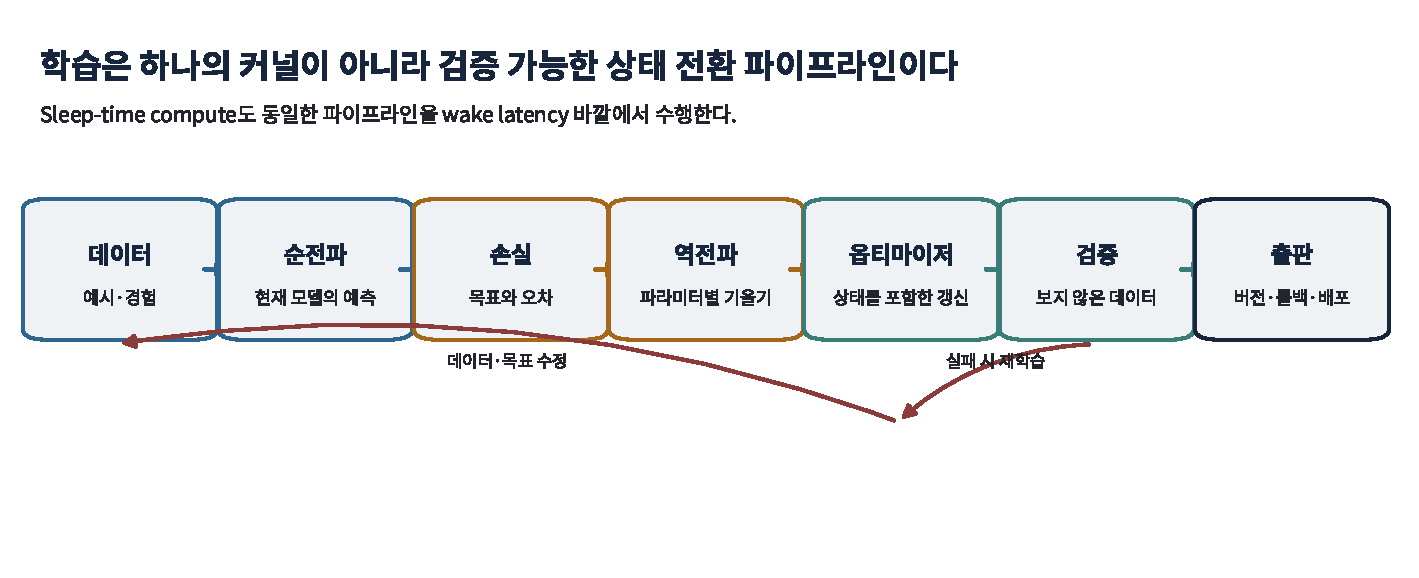
\includegraphics[width=\textwidth]{figures/learning-map.pdf}
  \caption{데이터에서 출판까지 이어지는 학습 상태 전환. Sleep-time compute는 이
  파이프라인의 일부를 응답 latency 경로 밖으로 옮기지만 검증 단계를 없애지 않는다.}
  \figsource{Original synthesis; context: SRC-STC-0030, SRC-STC-0014}{왼쪽의 데이터에서 오른쪽의 출판까지 일곱 상자가 화살표로 이어지고, 검증 실패 시 다시 데이터와 optimizer로 돌아간다.}
  \label{fig:bg-learning-map}
\end{figure}

\begin{keypoint}
학습 비용을 FLOPs만으로 세면 부족하다. 데이터 읽기, activation 보관, gradient와 optimizer
state, checkpoint 쓰기, validation inference, artifact 이동, rollback 보존까지가 한 번의
학습 상태 전환 비용이다.
\end{keypoint}

\chapter{순전파, 역전파, optimizer를 한 흐름으로 보기}
\label{bg:chapter-forward-backward}

\section{순전파는 값을 만들고, 역전파는 책임을 나눈다}

순전파는 layer를 따라 activation을 계산한다. 두 파라미터 모델
$f_{w,b}(x)=wx+b$에서 $x=2$, $y=10$, $w=3$, $b=1$이면 $\hat y=7$이다.
제곱손실은 $\ell=\frac12(7-10)^2=4.5$다. 출력 오차 $-3$이 $w$와 $b$에
각각 얼마나 책임이 있는지 계산하는 과정이 \concept{backpropagation}{역전파}다.

\concept{gradient}{기울기}는 손실의 국소 경사다.

\begin{align}
  \frac{\partial \ell}{\partial w} &= (wx+b-y)x = (-3)\cdot2=-6,\\
  \frac{\partial \ell}{\partial b} &= (wx+b-y)=-3.
  \label{eq:bg-two-parameter-gradient}
\end{align}

음의 기울기는 해당 파라미터를 늘리면 손실이 줄어드는 국소 방향임을 뜻한다. 학습률
$\eta=0.1$인 가장 단순한 gradient descent라면

\begin{equation}
  w' = w-\eta(-6)=3.6,\qquad b'=b-\eta(-3)=1.3
\end{equation}

이고 새 예측은 $8.5$, 손실은 $1.125$로 줄어든다. 이 예는 ``기울기가 기억 그 자체''가
아님을 보여 준다. 기울기는 지금 본 예에 대한 국소 변경 제안이고, 실제로 어떤 상태를
얼마나 바꿀지는 optimizer가 정한다.

\section{Optimizer는 update rule과 기억 상태를 가진다}

\concept{optimizer}{옵티마이저}는 기울기를 파라미터 변화로 바꾸는 알고리즘이다.
SGD는 현재 기울기를 직접 쓰지만, momentum은 과거 기울기의 이동평균을 유지한다.
Adam 계열은 보통 1차 모멘트 $m_t$와 2차 모멘트 $v_t$를 유지한다.
\concept{learning-rate}{학습률} $\eta$는 한 update에서 이 방향을 얼마나 크게 반영할지
정하는 scale이다.

\begin{align}
  m_t &= \beta_1m_{t-1}+(1-\beta_1)g_t,\\
  v_t &= \beta_2v_{t-1}+(1-\beta_2)g_t^2,\\
  \theta_{t+1} &= \theta_t-\eta
  \frac{\hat m_t}{\sqrt{\hat v_t}+\epsilon}.
  \label{eq:bg-adam}
\end{align}

$m_t$와 $v_t$가 \concept{optimizer-state}{옵티마이저 상태}다. parameter가 BF16으로
2 byte라 해도, 안정적인 학습을 위해 FP32 master weight, gradient, 두 moment를 보관하면
학습 중 persistent state는 parameter당 12--16 byte 수준이 될 수 있다. sharding과
8-bit optimizer가 이를 줄일 수 있지만, ``LoRA parameter가 작다''와 ``sleep job 전체
memory footprint가 작다''는 동일한 문장이 아니다. activation과 temporary buffer가 별도로
존재하기 때문이다.

\begin{table}[htbp]
\centering
\caption{추론과 학습 단계의 대표 상태}
\label{tab:bg-training-state}
\begin{tabularx}{\textwidth}{L{0.21\textwidth}YYY}
\toprule
상태 & 추론 & 학습 & 수명 \\
\midrule
model weights & 읽기 중심 & 읽기+갱신 & checkpoint 간 지속 \\
activations & 현재 token/layer & backward까지 보존 또는 재계산 & step 내부 \\
gradients & 없음 & trainable parameter마다 생성 & accumulation window \\
optimizer state & 없음 & momentum/variance/master copy & 여러 step 지속 \\
data state & prompt/KV & shuffle cursor, sampler, replay provenance & run 전체 \\
validation artifact & 선택적 & metric, failure slice, approval & release와 함께 지속 \\
\bottomrule
\end{tabularx}
\end{table}

\section{Activation memory와 checkpointing}

역전파는 각 layer의 입력 activation이 있어야 기울기를 계산하기 쉽다. 모든 activation을
HBM에 보관하면 빠르지만 memory를 많이 쓴다. 일부를 버리고 backward 때 다시 순전파하는
activation checkpointing은 compute를 늘려 memory를 줄인다. 따라서 같은 training FLOPs라
해도 sequence length, microbatch, layer checkpoint policy에 따라 HBM 요구량과 wall-clock이
달라진다.

Sleep-time training은 wake serving과 같은 GPU에서 돌아갈 수 있으므로 peak memory만이
문제가 아니다. checkpoint save가 storage bandwidth를 점유하고, parameter all-gather가
interconnect를 점유하며, validation이 inference slot을 가져간다. 좋은 스케줄러는 sleep job의
평균 utilization이 아니라 wake p99 latency를 보호해야 한다.

\section{Gradient accumulation과 effective batch}

한 번에 큰 batch가 HBM에 들어가지 않으면 여러 microbatch의 gradient를 더한 뒤 한 번
update한다. accumulation step을 $K$, microbatch 크기를 $B_\mu$라 하면 data-parallel replica
하나의 local effective batch는 $K B_\mu$다. replica가 $N$개이고 각 replica의 gradient를
동기화하면 global batch는 대략 $NKB_\mu$다.

하지만 token 길이가 다르면 ``문장 수 batch''와 ``token 수 batch''는 다르다. memory
consolidation에서는 긴 episode 몇 개가 gradient와 activation 대부분을 만들 수 있다.
따라서 scheduler는 examples/s보다 tokens/s, effective valid memories/s, update당 unique
provenance를 함께 기록해야 한다.

\begin{cautionbox}[작은 loss가 곧 좋은 장기기억은 아니다]
Training loss가 내려가도 replay 샘플의 중복, contamination, teacher 오류를 외웠을 수 있다.
반대로 old-task loss를 너무 강하게 고정하면 새 정보가 들어갈 공간이 사라진다. backward는
정확히 계산할 수 있지만, 무엇을 backward할지 정하는 목적과 데이터가 더 근본적인 문제다.
\end{cautionbox}

\section{Sleep-time operator로 번역하기}

Parametric sleep job을 한 번 실행한다고 하자. 먼저 selected episodes를 forward해 loss를
계산하고, backward로 gradient를 만든 뒤 optimizer가 adapter 또는 weights를 갱신한다.
그 다음 held-out memory query, old-capability suite, privacy probe, latency benchmark를
실행한다. 새 artifact가 모두 통과하면 version pointer를 바꾸고, 실패하면 이전 pointer를
유지한다. 이 순서에서 학습 kernel보다 중요한 시스템 계약은 다음과 같다.

\begin{enumerate}
  \item source episode와 gradient-producing example 사이의 provenance가 유지될 것,
  \item training state가 wake serving state와 원자적으로 분리될 것,
  \item validation 전 artifact가 사용자 traffic에 노출되지 않을 것,
  \item optimizer state를 재개할지 폐기할지 명시할 것,
  \item 삭제 요청 시 derived checkpoint와 adapter까지 추적할 수 있을 것.
\end{enumerate}

\chapter{배치, 샘플링, 검증: 데이터 흐름이 결과를 결정한다}
\label{bg:chapter-batch-evaluation}

\section{Batch는 단지 GPU를 채우는 단위가 아니다}

\concept{batch}{배치}는 한 update의 기울기를 추정하는 예시 집합이다. 전체 데이터의
평균 기울기를 매번 계산하는 대신 작은 subset의 평균을 사용하면 계산은 줄지만 추정에
noise가 생긴다. 적당한 noise는 평평한 해를 찾는 데 도움이 될 수 있고, 지나친 noise는
학습을 불안정하게 만든다. batch를 키우면 noise가 줄지만 activation memory와 통신량이
늘고, 같은 epoch에서 update 횟수가 줄어든다.

\concept{epoch}{에폭}은 데이터 전체를 대략 한 번 소비한 단위다. 고정 corpus에서는
직관적이지만, 계속 유입되는 agent experience에서는 명확한 epoch가 없다. 이때는 processed
tokens, unique episodes, wall-clock, user-days, consolidation cycles를 별도로 기록해야 한다.

\section{Sampling은 무엇을 기억하고 무엇을 잊을지 정한다}

\concept{sampling}{샘플링}은 다음 batch에 들어갈 데이터를 정한다. 균등 sampling은
흔한 사건을 반복 학습하고 rare but important event를 거의 보지 못할 수 있다. recency
sampling은 freshness를 높이지만 오래된 지식을 밀어낸다. surprise sampling은 모델이 크게
틀린 경험을 강조하지만 adversarial outlier와 noise에 취약하다. value sampling은 future
reuse가 높은 memory를 선택하려 하지만 그 value를 사전에 알기 어렵다.

Sleep system의 admission score를 개념적으로 다음처럼 둘 수 있다.

\begin{equation}
  s_i = \alpha u_i + \beta n_i + \gamma r_i
        -\delta q_i-\epsilon p_i,
  \label{eq:bg-admission-score}
\end{equation}

$u_i$는 관측된 utility, $n_i$는 novelty, $r_i$는 expected reuse, $q_i$는 품질 위험,
$p_i$는 privacy/governance 비용이다. 이것은 established formula가 아니라 scheduler가
숨겨 둔 판단을 명시적으로 드러내는 accounting form이다. 계수는 offline replay와
counterfactual evaluation으로 검증해야 한다.

\section{Training, validation, test의 역할}

\concept{validation-set}{검증 세트}는 hyperparameter, checkpoint, stopping 시점을 고르는 데
사용한다. \concept{test-set}{테스트 세트}는 선택을 마친 뒤 최종 일반화 성능을 추정한다.
test 결과를 보고 계속 모델을 수정하면 test도 사실상 validation이 되고, reported score는
낙관적으로 편향된다.

Memory system에서는 split 단위가 더 어렵다. 같은 사용자의 같은 사건을 paraphrase한 문장이
train과 test에 나뉘면 정보 누출이 생긴다. 공개 benchmark를 검색할 수 있는 agent는 test
question 자체를 sleep memory에 저장할 수 있다. 따라서 다음 split을 함께 고려해야 한다.

\begin{itemize}
  \item \textbf{time split}: 과거 episode로 학습하고 미래 interaction으로 평가한다.
  \item \textbf{entity split}: 특정 사람·프로젝트·도메인을 통째로 보존한다.
  \item \textbf{lineage split}: 동일 원문에서 파생된 summary와 paraphrase를 같은 split에 둔다.
  \item \textbf{policy split}: admission/eviction 정책의 학습 trace와 평가 trace를 분리한다.
  \item \textbf{contamination audit}: benchmark 문항이나 정답이 검색·기억에 들어왔는지 검사한다.
\end{itemize}

\section{Overfitting과 generalization}

\concept{overfitting}{과적합}은 training data에서 loss가 낮지만 새로운 data에서 성능이
나빠지는 현상이다. \concept{generalization}{일반화}는 보지 못한 상황에서도 배운 규칙이
유효한 정도다. 개인 memory에서는 ``같은 사실을 정확히 다시 말하기''와 ``그 사실을 새로운
작업에 적절히 적용하기''를 구분해야 한다. 전자는 retention, 후자는 transfer에 가깝다.

장기기억 평가는 최소 다섯 축이 필요하다.

\begin{enumerate}
  \item \textbf{write}: 올바른 정보가 destination state에 들어갔는가?
  \item \textbf{access}: 관련 query에서 그 정보가 실제 행동에 도달하는가?
  \item \textbf{retention}: 시간이 지나고 다른 update 뒤에도 유지되는가?
  \item \textbf{composition}: 다른 기억과 결합해 새로운 문제를 푸는가?
  \item \textbf{governance}: source를 추적하고 삭제·수정·rollback할 수 있는가?
\end{enumerate}

\begin{table}[htbp]
\centering
\caption{Sleep update의 평가 세트 예시}
\label{tab:bg-sleep-evaluation}
\begin{tabularx}{\textwidth}{L{0.20\textwidth}YYL{0.20\textwidth}}
\toprule
세트 & 포함 내용 & 실패가 뜻하는 것 & release gate \\
\midrule
new-memory query & 방금 통합한 사실·선호 & write/access 실패 & 핵심 recall 하한 \\
old-memory query & 이전 cycle의 기억 & catastrophic forgetting & regression 한도 \\
base capability & 범용 지식·추론·안전 & parametric side effect & non-inferiority \\
privacy/security & secret, poisoning, injection & 영구 오염 위험 & zero critical leak \\
systems & latency, bytes, energy, rollback & wake SLA/비용 실패 & budget ceiling \\
\bottomrule
\end{tabularx}
\end{table}

\section{통계적 유의성과 운영적 유의성}

표본이 크면 작은 차이도 통계적으로 유의할 수 있다. 하지만 0.1점 평균 향상이 adapter
수천 개, daily sleep cluster, 수십 TB write amplification을 정당화하지는 않는다. 반대로
희귀하지만 치명적인 deletion failure는 평균 score에 거의 보이지 않는다. 따라서 effect
size, confidence interval, tail risk, subgroup worst case, cost를 함께 보고한다.

\begin{keypoint}
Sleep-time compute의 올바른 test는 ``sleep 후 score가 올랐는가'' 하나가 아니다.
같은 future workload에서 external retrieval, longer context, cache, periodic refresh,
LoRA sleep을 동일한 data budget과 total cost로 비교해야 한다.
\end{keypoint}


\chapter{배포 전·후의 학습 regime 지도}
\label{bg:chapter-training-regimes}

\section{Regime를 네 질문으로 구분한다}

학습 이름이 많아 보이지만 네 질문으로 정리할 수 있다. (1) 언제 학습하는가, (2) 어떤
데이터를 쓰는가, (3) 어떤 상태가 바뀌는가, (4) 무엇이 serving artifact가 되는가. 이 네
항목이 같다면 이름이 달라도 시스템 workload는 비슷하고, 하나라도 다르면 compute와
governance가 달라진다.

\begin{figure}[htbp]
  \centering
  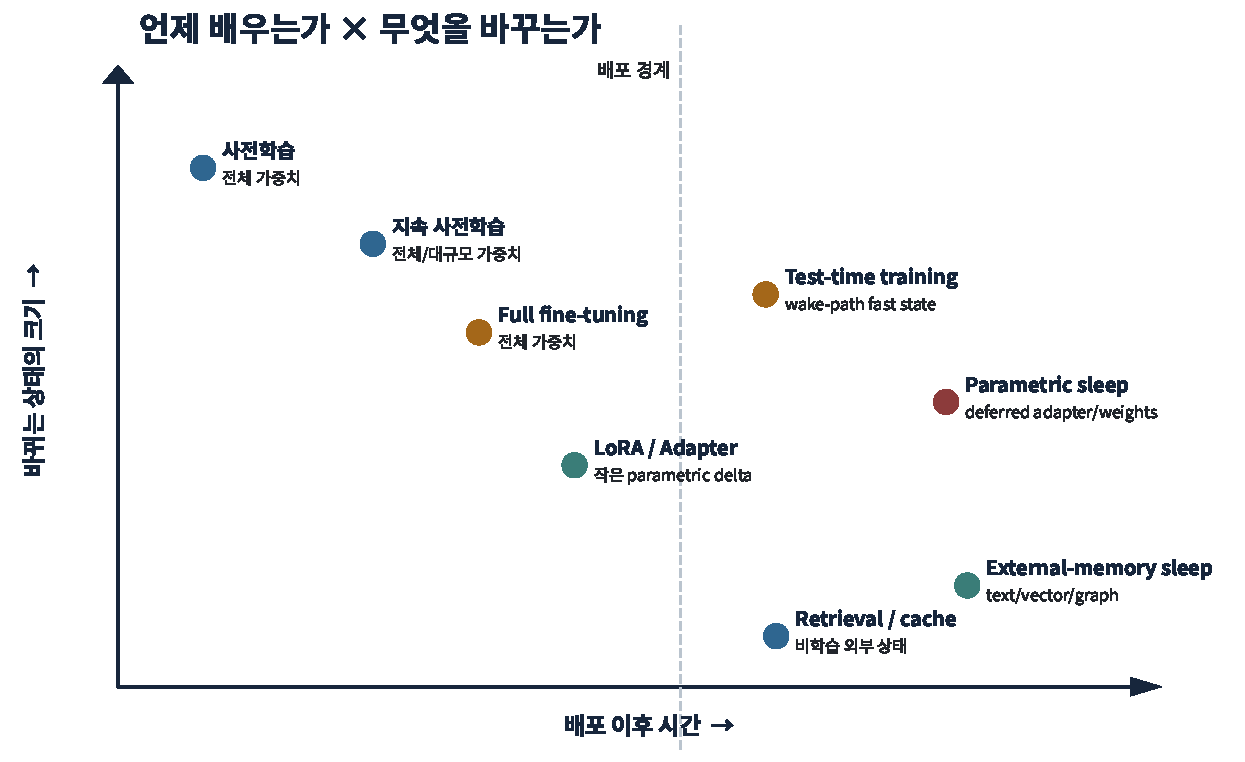
\includegraphics[width=0.95\textwidth]{figures/training-regimes.pdf}
  \caption{배포 시점과 변경 상태 크기로 본 training regime. Test-time training은 wake-path,
  sleep-time training은 deferred path에 놓이지만 둘 다 외부 기억과 parametric 상태를 선택할 수 있다.}
  \figsource{Original synthesis; SRC-STC-0014, SRC-STC-0021, SRC-STC-0030}{가로축은 배포 이후 시간, 세로축은 변경 상태 크기이고 사전학습, fine-tuning, LoRA, TTT, parametric sleep, external-memory sleep이 표시된다.}
  \label{fig:bg-training-regimes}
\end{figure}

\section{Pre-training과 continued pre-training}

\concept{pretraining}{사전학습}은 대규모 corpus에서 범용 representation과 생성 능력을
형성한다. language model은 보통 다음 token의 negative log-likelihood를 줄인다.

\begin{equation}
  \mathcal L_{\mathrm{LM}}(\theta)
  =-\sum_{t=1}^{T}\log p_\theta(x_t\mid x_{<t}).
  \label{eq:bg-lm-loss}
\end{equation}

한 번의 pre-training은 data curation, tokenizer, distributed optimizer, checkpoint,
evaluation이 결합된 장기 run이다. 모든 weight와 optimizer state가 sharding되고, 장애 시
재시작 가능한 checkpoint chain이 필요하다.

\concept{continued-pretraining}{지속 사전학습}은 이미 훈련된 model을 새 domain corpus나
최신 corpus로 계속 학습한다. 일반적으로 pre-training과 같은 self-supervised objective를
쓰지만 learning rate, data mixture, replay 비율을 조정한다. domain 지식은 늘 수 있으나
기존 능력과 언어 분포를 손상할 수 있어 base corpus replay와 broad evaluation이 필요하다.
Global knowledge refresh에는 유력하지만 per-user memory를 매 interaction마다 넣기에는
batching·privacy·rollback 단위가 너무 거칠 수 있다.

\section{Full fine-tuning과 instruction tuning}

\concept{fine-tuning}{미세조정}은 pretrained model을 더 좁은 데이터나 행동 목표에 맞게
추가 학습한다. full fine-tuning은 대부분 또는 모든 weight를 trainable하게 둔다. 작은
dataset에서도 높은 표현력을 갖지만, gradient·optimizer state·checkpoint가 full model
scale이고, 여러 사용자 variant를 독립 보관하기 어렵다.

\concept{instruction-tuning}{지시 튜닝}은 instruction--response pair로 원하는 task format과
behavior를 학습한다. 정답 token에 대한 supervised loss가 대표적이다. 답변 style과 tool
protocol을 형성하기 좋지만, interaction log를 그대로 정답으로 간주하면 사용자 오류와
assistant hallucination을 재학습할 수 있다. Sleep dataset은 raw transcript가 아니라
verifier를 통과한 target과 negative example을 포함해야 한다.

\section{Preference optimization}

\concept{preference-optimization}{선호 최적화}는 두 출력 중 어느 것이 더 나은지에 대한
preference를 사용한다. reward model을 따로 학습하고 policy를 RL로 최적화할 수도 있고,
chosen/rejected pair에서 직접 loss를 만들 수도 있다. 중요한 것은 algorithm 이름보다
reference behavior, preference provenance, distribution shift다.

개인화 sleep에서는 ``사용자가 한번 수정했다''는 사건을 영구 선호로 확대하면 위험하다.
상황적 요청, 장기 선호, 조직 policy를 구분해야 한다. preference update는 probability를
바꾸기 때문에 사실 memory와 달리 정확한 source sentence 하나로 rollback하기 어렵다.

\begin{table}[htbp]
\centering
\caption{대표 training regime의 상태와 비용}
\label{tab:bg-training-regimes}
\small
\begin{tabularx}{\textwidth}{L{0.16\textwidth}L{0.17\textwidth}L{0.18\textwidth}YY}
\toprule
Regime & 주 데이터 & Trainable state & Serving artifact & 주요 실패 \\
\midrule
pre-training & web/code/multimodal corpus & 전체 weights + optimizer & base checkpoint & bias, contamination, huge cost \\
continued PT & domain/latest corpus + replay & 전체 또는 대규모 weights & refreshed checkpoint & domain drift, forgetting \\
full FT & labeled task/user data & 전체 weights & full variant & interference, storage explosion \\
instruction tuning & instruction-response & 전체 또는 PEFT & aligned checkpoint/adapter & imitation of bad targets \\
preference opt. & comparisons/reward & policy + optional reward model & aligned policy & reward hacking, preference drift \\
LoRA/adapter & task/user examples & 작은 delta/module & base + delta & adapter conflict, base churn \\
TTT & current input/stream & fast weights/state & session state & latency, instability \\
sleep training & accumulated episodes & chosen destination state & validated next version & stale data, rollback, fleet cost \\
\bottomrule
\end{tabularx}
\end{table}

\section{Sleep-time은 새로운 objective가 아니라 lifecycle 축이다}

Sleep-time compute는 특정 optimizer나 architecture의 이름이 아니다. 같은 LoRA update도
response를 만들기 전에 current query로 수행하면 test-time training이고, response 이후
여러 episode를 정리해 다음 session의 adapter를 만들면 sleep-time training이다. 반대로
background process가 text summary와 graph edge만 갱신한다면 training kernel 없이도 sleep
lifecycle에 속한다.

따라서 infra를 분류할 때 ``training cluster인가 inference cluster인가''만 묻지 않는다.
wake critical path, deferred transformation path, persistent state destination, validation and
publication plane을 따로 본다. 이 구분이 있어야 sleep job을 spare GPU에 단순 배치하는 접근과
state-aware lifecycle system을 구별할 수 있다.

\chapter{지도 신호, 자기지도, representation과 언어모델 loss}
\label{bg:chapter-supervision}

\section{정답은 어디서 오는가}

\concept{supervision}{지도 신호}는 입력에 대해 원하는 target이나 비교를 제공한다.
image label, 정답 문장, tool execution result, 사람 preference가 모두 supervision이다.
정답 비용이 높고 누락·편향이 존재하므로 data provenance가 중요하다.

\concept{self-supervision}{자기지도학습}은 raw data 안에서 target을 만든다. 다음 token 예측은
앞 token을 input, 실제 다음 token을 target으로 사용한다. 별도 사람이 모든 문장을 label하지
않아도 scale할 수 있지만, 데이터가 사실인지 안전한지는 보장하지 않는다. Sleep transcript를
그대로 next-token target으로 쓰면 model error와 prompt injection도 학습 대상이 될 수 있다.

\section{Representation은 저장소와 다르다}

\concept{representation}{표현}은 input을 후속 계산에 유용한 vector 또는 state로 바꾼
것이다. representation 안에 정보가 통계적으로 존재하는 것과, model이 필요한 query에서
그 정보를 꺼내 행동에 쓰는 것은 다르다. linear probe가 fact를 읽어도 generation path가
접근하지 못할 수 있다. 그래서 parametric memory의 capacity는 단순 bit encoding, probe
decodability, behavioral access, composition을 나눠 측정해야 한다.

External vector memory도 마찬가지다. embedding space에 가까운 record가 존재해도 retriever가
top-$k$에 넣지 못하거나, generator가 context를 무시하면 end-to-end memory는 실패한다.
Memory medium에 상관없이 write, address, read, use의 네 단계를 구분한다.

\section{Logit, softmax, cross-entropy}

언어모델의 마지막 layer는 vocabulary 각 token에 \concept{logit}{로짓} $z_i$를 준다.
\concept{softmax}{소프트맥스}는 이를 확률로 바꾼다.

\begin{equation}
  p_i=\frac{\exp(z_i)}{\sum_j\exp(z_j)}.
  \label{eq:bg-softmax}
\end{equation}

정답 token이 $y$일 때 \concept{cross-entropy}{교차엔트로피}는
$\ell=-\log p_y$다. 정답 확률이 1에 가까우면 0에 가까워지고, 낮으면 커진다. 이 loss는
모든 오답 token을 동일한 의미로 보지 않는다. 확률 분포 전체를 통해 gradient가 흐른다.

예를 들어 vocabulary가 세 token이고 logit이 $(2,1,0)$이면 softmax 확률은 대략
$(0.665,0.245,0.090)$이다. 첫 token이 정답이면 loss는 약 $0.408$, 셋째가 정답이면
약 $2.408$이다. 그러나 ``서울은 한국의 수도''를 맞히는 token loss와 사용자 개인정보를
노출하는 token loss는 제품 위험이 다르다. objective weighting과 evaluation이 이를 반영해야
한다.

\section{Mask와 sequence-level objective}

LLM training에서는 padding token, prompt token, tool output 중 어느 token에 loss를 줄지
mask로 결정한다. Instruction tuning에서 user prompt까지 모방 loss를 주면 user 발화를
assistant가 생성하려 할 수 있다. tool trace의 private field를 mask하지 않으면 secret을
학습할 수 있다.

Token loss만으로 sequence의 factual consistency나 task success를 직접 표현하기 어렵다.
verifier score, execution success, preference loss, contrastive loss를 결합할 수 있지만 objective가
많아질수록 gradient conflict와 weight selection 문제가 생긴다.

\begin{equation}
  J = \lambda_{\mathrm{new}}L_{\mathrm{new}}
      +\lambda_{\mathrm{replay}}L_{\mathrm{old}}
      +\lambda_{\mathrm{safety}}L_{\mathrm{safety}}
      +\lambda_{\mathrm{anchor}}D(f_\theta,f_{\theta_0}).
  \label{eq:bg-multiobjective}
\end{equation}

$D$는 old model과의 behavior 차이를 제한한다. 계수 하나를 바꾸면 무엇을 ``기억''으로
보존하는지가 달라진다. Sleep controller는 data selection뿐 아니라 loss mixture까지 policy로
관리할 수 있지만, 그 policy 자체가 또 하나의 학습·검증 대상이 된다.

\section{Systems 관점: data transformation도 compute다}

Training FLOPs 이전에 transcript parsing, PII filtering, deduplication, semantic clustering,
negative construction, teacher generation, verifier execution이 있다. External-memory sleep은
이 transformation만 수행하고 weight backward는 하지 않을 수 있다. 그래서 background
synthesis도 중요한 sleep-time compute다. GPU FLOPs가 작아도 graph update와 vector index
rewrite가 storage-bound일 수 있으며, source history가 길수록 read amplification이 커진다.

\begin{cautionbox}
Self-generated target은 무료 data가 아니다. teacher error, confirmation bias, model collapse,
benchmark leakage를 추적해야 한다. 실제 사용자/환경 관측이라는 anchor와 recursive generation
depth를 provenance에 남기지 않으면 나중에 품질 저하의 원인을 찾을 수 없다.
\end{cautionbox}


\chapter{Distillation: 큰 경험을 작은 상태로 옮기기}
\label{bg:chapter-distillation}

\section{교사와 학생}

\concept{distillation}{지식 증류}는 \concept{teacher-model}{교사 모델}이 제공한 output
distribution, rationale, feature, selected answer를 \concept{student-model}{학생 모델}이
모방하도록 학습하는 방식이다. 교사가 더 크거나 더 많은 context를 사용할 수 있고, 학생은
작거나 latency가 낮을 수 있다. Sleep context에서는 긴 episodic history를 짧은 memory,
adapter, 작은 model로 압축하는 operator로 이해할 수 있다.

Hard target은 교사의 최고 확률 token 하나만 사용한다. Soft target은 전체 분포를 사용해
두 번째·세 번째 선택지에 대한 정보도 전달한다. \concept{temperature}{온도} $T$를 적용하면

\begin{equation}
  p_i^{(T)}=\frac{\exp(z_i/T)}{\sum_j\exp(z_j/T)}.
\end{equation}

$T>1$에서 분포가 평평해져 relative preference가 더 드러난다. 학생 분포 $q$와 교사 분포
$p$ 사이 \concept{kl-divergence}{KL 발산}을 줄일 수 있다.

\begin{equation}
  D_{\mathrm{KL}}(p\Vert q)=\sum_i p_i\log\frac{p_i}{q_i}.
  \label{eq:bg-kl}
\end{equation}

KL은 대칭 거리가 아니다. 어떤 방향을 쓰는지에 따라 mode covering과 mode seeking 특성이
달라진다. 실제 distillation loss는 hard label loss와 soft loss를 섞는다.

\begin{equation}
  L=\alpha L_{\mathrm{hard}}+(1-\alpha)T^2
  D_{\mathrm{KL}}(p_T\Vert q_T).
  \label{eq:bg-distill-loss}
\end{equation}

\section{Memory consolidation으로서 distillation}

긴 history를 매번 prompt에 넣는 대신 teacher가 충분한 context와 retrieval을 사용해 reusable
summary나 strategy를 만든다. destination에 따라 세 종류로 나뉜다.

\begin{enumerate}
  \item \textbf{External distillation}: episode를 concise text, vector prototype, graph fact로 바꾼다.
  \item \textbf{Adapter distillation}: teacher의 behavior를 LoRA나 adapter에 학습한다.
  \item \textbf{Model distillation}: 여러 cycle의 memory를 base model weights로 통합한다.
\end{enumerate}

첫 번째는 provenance와 수정이 쉽고 inference 때 retrieval cost가 남는다. 두 번째는 repeated
query의 retrieval cost를 줄일 수 있지만 base model compatibility와 adapter routing이 필요하다.
세 번째는 access latency가 가장 낮을 수 있으나 interference, deletion, rollback cost가 가장
크다.

\section{무엇이 압축 과정에서 사라지는가}

Distillation은 loss가 중요하게 보는 behavior만 보존한다. rare exception, uncertainty,
source wording, provenance는 teacher output에 드러나지 않으면 사라진다. 외부 summary가
``사용자는 항상 아침 운동을 선호한다''고 일반화했지만 원 episode가 ``이번 주만''이었다면
identity drift가 발생한다.

세 가지 검증을 분리한다.

\begin{itemize}
  \item \textbf{fidelity}: teacher와 student가 같은 query distribution에서 얼마나 같은가?
  \item \textbf{utility}: teacher와 달라도 downstream task를 실제로 더 잘 푸는가?
  \item \textbf{provenance preservation}: output의 각 claim을 source episode로 되돌릴 수 있는가?
\end{itemize}

Fidelity가 너무 높으면 teacher 오류까지 복사한다. utility만 최적화하면 근거 없는 shortcut을
배울 수 있다. provenance는 loss 한 항으로 쉽게 보장되지 않으므로 external metadata와
release gate가 필요하다.

\section{Recursive distillation과 model collapse}

Sleep cycle $k$의 output이 cycle $k+1$의 training data가 되면 recursive depth가 증가한다.
실제 data anchor가 줄고 생성 data만 반복되면 distribution tail이 사라질 수 있다
\parencite{shumailov2024collapse}. 반면 real data를 계속 누적하는 조건에서는 collapse가
필연적이지 않을 수 있다. 따라서 synthetic 여부의 이분법 대신 각 item에
origin, teacher version, recursive depth, real-evidence links를 기록한다.

\begin{table}[htbp]
\centering
\caption{Sleep distillation destination의 차이}
\label{tab:bg-distillation-destinations}
\begin{tabularx}{\textwidth}{L{0.19\textwidth}YYYY}
\toprule
Destination & update 비용 & wake 비용 & 수정/삭제 & 대표 위험 \\
\midrule
text summary & 낮음--중간 & retrieval/context & 쉬움 & over-compression \\
vector prototype & 중간 & ANN search & 중간 & embedding drift \\
temporal graph & 중간--높음 & traversal + context & 비교적 쉬움 & conflict/edge explosion \\
LoRA/adapter & training 필요 & routing + matmul & version rollback 가능 & conflict/base churn \\
full weights & 가장 높음 & 낮을 수 있음 & 가장 어려움 & interference/unlearning \\
\bottomrule
\end{tabularx}
\end{table}

\begin{keypoint}
Distillation은 기억을 ``옮기는'' 마법이 아니라 task distribution이 정한 정보만 보존하는
lossy compression이다. Sleep system은 압축률뿐 아니라 삭제 가능한 provenance와 later
utility를 함께 최적화해야 한다.
\end{keypoint}

\chapter{PEFT, LoRA, adapter, MoE: 얼마나 작은 상태를 바꿀 것인가}
\label{bg:chapter-peft}

\section{Trainable state를 줄이는 이유}

Full fine-tuning은 모든 weight에 gradient와 optimizer state를 만든다. 사용자·도메인별
variant가 많아지면 compute뿐 아니라 checkpoint storage와 model residency가 폭증한다.
\concept{peft}{PEFT}는 base model을 고정하고 작은 subset 또는 추가 module만 학습해 이
비용을 줄인다. 하지만 trainable parameter 비율과 total system cost를 구분해야 한다.
Base weight는 여전히 forward/backward에 참여하며 activation과 input data를 읽는다.

\concept{trainable-state}{학습 가능 상태}는 gradient를 받아 갱신되는 상태다. 반면
\concept{serving-artifact}{서빙 산출물}은 실제 wake inference에 배포되는 base checkpoint,
delta, routing table, index의 조합이다. Sleep job이 작은 delta만 만들더라도 수백만 사용자의
delta를 catalog, cache, prefetch, revoke하는 serving system은 클 수 있다.

\section{LoRA의 최소 수식}

\concept{lora}{LoRA}는 고정 weight $W_0\in\mathbb{R}^{d_{out}\times d_{in}}$에 low-rank
delta를 더한다 \parencite{hu2021lora}.

\begin{equation}
  W = W_0 + \Delta W,
  \qquad \Delta W = \frac{\alpha}{r}BA,
  \label{eq:bg-lora}
\end{equation}

$A\in\mathbb{R}^{r\times d_{in}}$, $B\in\mathbb{R}^{d_{out}\times r}$이고
$r\ll \min(d_{in},d_{out})$다. full matrix의 $d_{out}d_{in}$개 대신
$r(d_{in}+d_{out})$개를 학습한다. 예를 들어 $d_{in}=d_{out}=4096$, $r=16$이면 한
projection의 trainable parameter는 약 16.8M에서 131K로 줄어 약 128배 작다.

그러나 다음 비용은 남는다.

\begin{itemize}
  \item base layer를 통과하는 forward와 backward activation,
  \item LoRA A/B gradient와 optimizer state,
  \item 여러 target module(Q/K/V/O, MLP)에 대한 delta,
  \item user/domain별 adapter 저장·인덱싱·authentication,
  \item base checkpoint가 바뀔 때 compatibility 재검증,
  \item 여러 adapter를 합성할 때 발생하는 conflict.
\end{itemize}

\section{Adapter module과 routing}

\concept{adapter}{어댑터}는 layer 사이에 작은 bottleneck module을 추가한다. 전형적인 형태는

\begin{equation}
  h' = h + W_{up}\,\sigma(W_{down}h)
\end{equation}

이다. Base를 고정할 수 있고 adapter별 version이 명확하다. 대신 inference graph에 추가
operator가 생기며, 어떤 adapter를 언제 load할지 routing해야 한다. adapter가 HBM에 없으면
storage-to-HBM load latency가 first-token latency에 나타날 수 있다. 여러 작은 adapter가
random access workload를 만들면 총 byte보다 IOPS와 metadata lookup이 병목일 수 있다.

\section{Mixture of Experts는 PEFT와 다른 축이다}

\concept{mixture-of-experts}{Mixture of Experts(MoE)}는 token마다 router가 일부 expert만
활성화하는 sparse architecture다. 전체 parameter capacity는 크지만 active FLOPs는 일부다.
MoE가 자동으로 개인 memory system이 되는 것은 아니다. Expert가 pretrained/fixed인지,
sleep 중 새 expert를 추가하는지, user-specific routing을 학습하는지에 따라 의미가 달라진다.

Sleep-time 관점에서 MoE는 세 기회를 준다. (1) stable domain knowledge를 expert로 격리,
(2) base 전체가 아닌 selected expert만 update, (3) cold expert를 lower memory tier에 offload.
동시에 all-to-all communication, expert imbalance, cache miss, expert proliferation이라는 시스템
문제를 만든다.

\begin{table}[htbp]
\centering
\caption{Full FT, LoRA, adapter, external memory의 비교}
\label{tab:bg-peft-comparison}
\small
\begin{tabularx}{\textwidth}{L{0.15\textwidth}YYYYY}
\toprule
방법 & trainable state & optimizer state & wake access & rollback & 핵심 병목 \\
\midrule
Full FT & 전체 weight & 전체 규모 & 직접 weight & checkpoint 단위 & HBM/compute/interference \\
LoRA & low-rank delta & delta 규모 & base+delta matmul & delta version & adapter catalog/cache \\
Adapter & 작은 module & module 규모 & extra module & module version & routing/load latency \\
MoE update & selected experts & expert subset & sparse routing & expert/version & all-to-all, imbalance \\
External memory & text/vector/graph & 선택적 & retrieval+context & record/version & index, context pollution \\
\bottomrule
\end{tabularx}
\end{table}

\section{Selective promotion이라는 hybrid}

모든 episode를 weight로 넣지 않고 external system-of-record에 먼저 보관한다. 충분한 future
reuse, stability, cross-user generality, safety evidence가 쌓인 item만 adapter나 periodic global
refresh로 승격한다. 이 구조는 raw episode의 provenance와 delete를 유지하면서 high-reuse
knowledge의 repeated retrieval cost를 줄일 수 있다.

Promotion break-even의 최소 형태는 다음과 같다.

\begin{equation}
  C_{\mathrm{compile}}+C_{\mathrm{validate}}+C_{\mathrm{store}}
  < N_{\mathrm{future}}\left(C_{\mathrm{retrieve}}-C_{\mathrm{parametric\ access}}\right).
  \label{eq:bg-promotion-break-even}
\end{equation}

$N_{\mathrm{future}}$가 작거나 base model churn이 빠르면 승격은 손해다. 따라서 adapter는
``항상 더 효율적인 기억''이 아니라 later reuse가 충분할 때만 이기는 compiled cache에
가깝다.

\begin{cautionbox}[작은 delta의 함정]
LoRA file이 작다는 사실만으로 user-specific parametric memory가 scale한다고 결론 내릴 수
없다. adapter 수, active working set, load pattern, validation cost, base-version migration,
deletion SLA를 함께 측정해야 한다.
\end{cautionbox}

\IfFileExists{sections/08-data-augmentation-replay.tex}{\chapter{Sleep이 먹는 것: data curation, augmentation, replay}
\label{bg:chapter-data-replay}

Sleep-time compute가 training이라면 첫 질문은 ``어떤 optimizer를 쓸까''가 아니라
``어떤 경험을 학습 가능한 증거로 만들까''다. Wake log에는 사용자 발화, model response,
tool result, correction, 반복 조회, 실패 trace가 섞여 있다. 이들을 그대로 next-token data로
넣으면 개인 식별 정보, 틀린 model output, 중복된 쉬운 예, 시간 순서가 깨진 사실이 모두 같은
가중치로 학습된다. 따라서 sleep pipeline의 품질 상한은 대개 data plane에서 정해진다.

\section{Log와 training example은 다르다}

\concept{data-curation}{데이터 큐레이션}은 후보 경험을 수집하고 정규화하며 중복을 제거하고,
목표·권리·민감도·시간 범주를 부여하는 전 과정이다. \concept{data-filtering}{데이터 필터링}은
그중 정해진 기준으로 남길 것과 제외할 것을 가르는 단계다. 둘을 분리해야 ``수집은 했지만
학습에는 쓰지 않음'', ``외부 기억에는 보존하지만 parametric update에는 금지'' 같은 결정을
표현할 수 있다.

한 sleep example $e_i$를 최소한 다음 record로 본다.

\begin{equation}
e_i=(x_i, y_i, t_i, u_i, s_i, q_i, r_i, p_i, v_i),
\end{equation}

여기서 $x_i$는 입력 context, $y_i$는 목표 또는 preference, $t_i$는 event time, $u_i$는
user/tenant scope, $s_i$는 source type, $q_i$는 quality와 uncertainty, $r_i$는 retention/rights,
$p_i$는 provenance pointer, $v_i$는 생성한 model·tool version이다. 실제 시스템에서는 원문과
이 record를 분리해 저장할 수 있다. 원문 삭제 요청을 처리하려면 record가 어느 artifact와
update에 기여했는지도 이어져야 한다.

\concept{provenance}{출처 추적성}은 단순 URL 열이 아니다. ``원본 event $\rightarrow$
정제 record $\rightarrow$ replay batch $\rightarrow$ checkpoint $\rightarrow$ serving version''을
역추적할 수 있어야 한다. provenance가 없으면 잘못된 기억을 발견해도 external index 한 row만
지우면 되는지, LoRA를 폐기해야 하는지, base model을 다시 만들어야 하는지 판단할 수 없다.

\begin{table}[htbp]
\centering
\caption{Wake event를 sleep data로 바꿀 때 필요한 gate}
\label{tab:bg-data-gates}
\small
\begin{tabularx}{\textwidth}{p{0.16\textwidth} X X}
\toprule
Gate & 묻는 질문 & 실패 시 기본 동작 \\
\midrule
scope & 누구의 기억이며 어느 tenant에서만 유효한가? & global 학습 금지, 격리 저장 \\
grounding & correction이나 fact가 신뢰 가능한 source에 연결되는가? & 외부 후보로 격하 또는 제외 \\
temporal & 언제부터 언제까지 참이며 newer record와 충돌하는가? & time interval과 supersession edge 기록 \\
rights/privacy & 저장·재생·가중치 반영·장기 보존 권한이 각각 있는가? & 허용된 destination만 사용 \\
difficulty & 모델이 이미 맞히는 중복 easy example인가? & down-sample 또는 대표 예만 보존 \\
contamination & validation/test 또는 비공개 benchmark 정답이 섞였는가? & quarantine, 평가 집합 재구성 \\
\bottomrule
\end{tabularx}
\end{table}

\section{Augmentation은 의미를 보존한다는 가정이다}

\concept{data-augmentation}{데이터 증강}은 한 예시를 여러 변형으로 늘리는 기법이지만,
핵심은 ``이 변환 아래 목표가 변하지 않는다''는 invariance 가정이다. 이미지 회전처럼 명확한
경우도 있지만 memory data에서는 더 위험하다. 발화를 paraphrase하면 표현 다양성은 늘지만
negation, 날짜, actor, uncertainty가 바뀔 수 있다. context를 잘라내면 정답은 남아 보여도
근거와 privacy scope가 사라질 수 있다.

Sleep용 augmentation은 세 층으로 나누면 안전하다.

\begin{enumerate}
  \item \textbf{surface augmentation}: 표현·순서·format을 바꾸되 entity, time, polarity,
        provenance를 보존한다.
  \item \textbf{contrast construction}: 헷갈리는 old/new fact, 같은 이름의 다른 사람,
        허용/금지 scope를 쌍으로 만들어 decision boundary를 학습한다.
  \item \textbf{counterfactual probe}: 목표 자체를 학습시키기보다 모델이 evidence 없이
        외운 답을 내는지 평가한다. training set과 validation set을 섞지 않는다.
\end{enumerate}

\concept{synthetic-data}{합성 데이터}는 teacher model, simulator, rule로 만든 예시다. 긴
episode를 question--answer pair로 변환하거나 드문 failure를 증폭하는 데 유용하지만, 생성자의
오류와 표현 편향도 함께 복제한다. recursive distillation에서 생성 data가 다시 다음 cycle의
teacher data가 되는 깊이를 record하고, real-evidence anchor를 일정 비율 유지해야 하는 이유가
여기에 있다 \parencite{shumailov2024collapse}.

\section{Replay: 과거를 다시 보여 주는 가장 직접적인 기준선}

\concept{replay-buffer}{리플레이 버퍼}는 과거 경험 일부를 다시 학습시키기 위한 제한된 저장소다.
새 batch $B_{new}$만 학습하지 않고 replay sample $B_{old}$를 섞으면

\begin{equation}
\mathcal{L}_{sleep}=\lambda_{new}\mathcal{L}(B_{new})+
\lambda_{old}\mathcal{L}(B_{old})+lambda_{safe}\mathcal{L}(B_{safety})
\end{equation}

처럼 plasticity와 retention을 직접 trade-off할 수 있다. 작은 episodic memory도 forgetting을
줄이는 강한 baseline이 될 수 있으며 \parencite{chaudhry2019tiny}, class prototype에 가까운
대표 예를 유지하는 방식도 쓰인다 \parencite{rebuffi2017icarl}. 그러나 buffer가 raw episode를
보존하면 저장·privacy 비용이 크고, random sampling은 다수 사용자의 반복 패턴이 희귀하지만
중요한 경험을 밀어낸다.

\concept{coreset}{코어셋}은 전체 데이터의 loss나 representation을 작은 weighted subset으로
근사하려는 관점이다. Sleep system에서는 단순 diversity 외에도 다음 utility를 함께 본다.

\begin{equation}
U(e)=\alpha N(e)+\beta E(e)+\gamma F(e)+\delta R(e)
-\eta C_{store}(e)-\zeta C_{risk}(e),
\end{equation}

$N$은 novelty, $E$는 evidence quality, $F$는 예상 future reuse, $R$은 forgetting 방지 기여다.
이 점수는 established formula가 아니라 controller를 설계하기 위한 decomposition이다. 각 항의
scale과 label delay가 다르므로 하나의 숫자로 만들기 전에 raw features와 의사결정 이유를 남긴다.

\concept{generated-replay}{생성 리플레이}는 raw 과거를 전부 저장하는 대신 generator가 과거
분포를 복원하도록 한다 \parencite{shin2017dgr}. 저장 bytes를 줄일 수 있지만 generator 자체도
잊고, 원본 provenance를 잃으며, tail을 평탄화할 수 있다. 따라서 ``raw replay 대 generated
replay''는 어느 하나를 고르는 문제가 아니라 민감한 원문, 검증된 canonical fact, 일반 skill
pattern에 서로 다른 retention을 주는 tiering 문제다.

\begin{keypoint}[Sleep dataset의 최소 산출물]
Sleep job 입력은 folder 하나가 아니라 immutable dataset manifest여야 한다. manifest에는 source
snapshot, filter version, included/excluded count와 reason, tenant/time scope, dedup cluster,
augmentation lineage, train/validation split, hash, expiry가 포함된다. 같은 checkpoint를 다시 만들 수
없다면 rollback도 감사도 불가능하다.
\end{keypoint}

\section{평가 누수와 시간 누수}

개인화 memory에서는 random split이 특히 위험하다. 같은 episode의 paraphrase가 train과 validation에
나뉘면 memorization을 generalization으로 오해한다. 미래 correction이 과거 시점 평가 입력에 들어가면
temporal leakage가 생긴다. 권장 split unit은 token이 아니라 user, episode, entity thread, time window다.
평가는 ``현재 사실 회상'', ``과거 시점 질의'', ``다른 user로의 비누출'', ``삭제 후 비회상''을 분리한다.

Sleep-time compute에서 data volume은 공짜 scaling 축이 아니다. 중복 experience를 더 많이 replay하면
FLOPs는 늘지만 effective evidence는 거의 늘지 않는다. 그래서 future scaling law의 독립변수는 raw
token 수보다 provenance-weighted novel evidence, replay diversity, recursive depth, validation coverage에
가까워야 한다.
}{}
\IfFileExists{sections/09-continual-learning.tex}{\chapter{계속 배우면서 잊지 않기: continual learning의 문제 설정}
\label{bg:chapter-continual-learning}

\concept{continual-learning}{지속학습}은 데이터 분포가 한 번에 주어지지 않고 시간에 따라 도착할 때,
새 능력을 획득하면서 과거 능력도 유지하려는 설정이다. Sleep-time compute가 매일 또는 매 session 뒤
모델을 갱신한다면 자연스럽게 continual learning 문제가 된다. 단, 실제 agent stream은 benchmark처럼
``Task 1 종료, Task 2 시작'' 표지를 주지 않으며 사용자·사실·도구·정책 변화가 겹친다.

\section{왜 새 학습이 과거 능력을 지우는가}

한 파라미터 $\theta_j$가 과거 task A와 새 task B에 동시에 쓰인다고 하자. B의 loss를 줄이는 gradient가
A의 loss를 늘리는 방향이면 같은 update가 양쪽에 반대 효과를 낸다. 새 data만 반복하면 optimizer는
과거 data를 보지 못하므로 그 손실 증가를 감지하지 못한다. 이를 \concept{catastrophic-forgetting}{파국적
망각}이라 부른다. ``parameter capacity가 꽉 찼다''는 말과 같지는 않다. 충분한 파라미터가 있어도
optimization path와 sampling 때문에 잊을 수 있고, 반대로 작은 모델도 잘 선택한 replay와 isolation으로
오래 유지할 수 있다.

\concept{stability-plasticity}{안정성–가소성 dilemma}는 두 오류를 함께 본다.

\begin{itemize}
  \item 안정성만 높이면 이전 기능은 보존하지만 새로운 correction과 변화에 적응하지 못한다.
  \item 가소성만 높이면 최신 session에는 잘 맞지만 오래된 skill과 safety behavior가 무너진다.
\end{itemize}

Complementary Learning Systems 관점은 빠른 episodic store와 느린 cortical integration을 분리하고,
interleaved replay로 새 경험을 기존 구조에 통합한다 \parencite{mcclelland1995cls}. 이는 biological
sleep을 그대로 구현하라는 처방이 아니라, fast store가 제공하는 sparse episode와 slow learner가
요구하는 mixed training distribution이 다르다는 설계 basis다.

\section{성능 행렬로 retention과 transfer를 분리한다}

$R_{i,j}$를 task $j$까지 학습한 뒤 task $i$에서 측정한 성능이라 하자. 마지막 시점 평균 성능은

\begin{equation}
A_T=\frac{1}{T}\sum_{i=1}^{T}R_{i,T}
\end{equation}

이고, task $i$가 과거에 기록한 최고 성능에서 마지막 성능이 떨어진 양은

\begin{equation}
F_T=\frac{1}{T-1}\sum_{i=1}^{T-1}
\left(\max_{j\in\{i,\ldots,T-1\}}R_{i,j}-R_{i,T}\right)
\end{equation}

로 측정할 수 있다. \concept{backward-transfer}{후방 전이}는 새 학습이 과거 task를 개선하면 양수,
악화하면 음수인 방향성 지표다 \parencite{lopezpaz2017gem}. 평균 정확도 하나는 latest adaptation과
retention을 섞으므로 sleep controller 비교에 부족하다.

LLM memory에는 task label 대신 evaluation slice를 둔다. 예를 들어 user preference, stable personal
fact, time-varying fact, tool procedure, safety refusal, general capability, privacy non-leakage를 별도
행으로 만든다. 각 sleep version 뒤 이 행렬을 다시 측정해야 어느 축에서 얻고 잃었는지 보인다.

\begin{figure}[htbp]
  \centering
  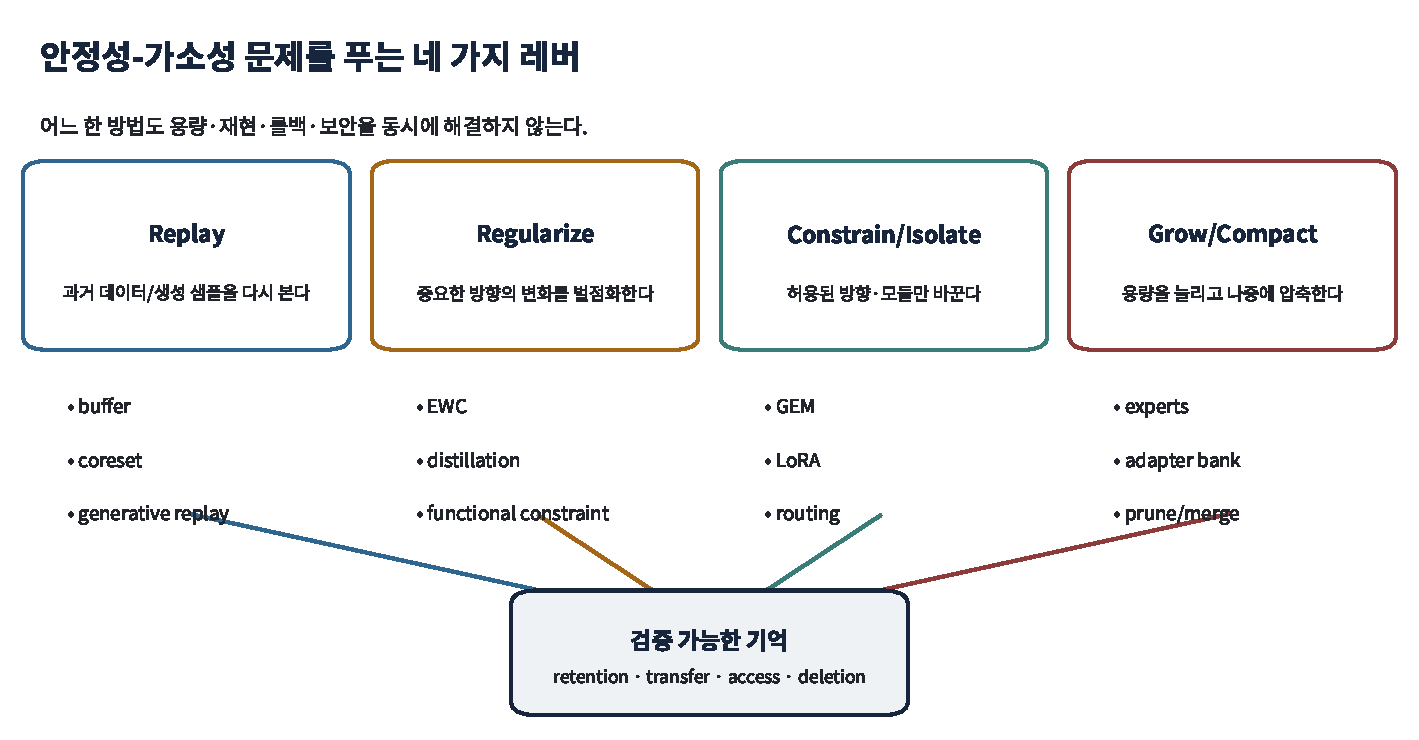
\includegraphics[width=0.95\textwidth]{figures/continual-learning-map.pdf}
  \caption{Continual-learning 방법을 replay, regularization, constraint/isolation,
  growth/compaction으로 나눈 지도. 네 계열 모두 별도 retention 평가와 publication gate가 필요하다.}
  \figsource{Original synthesis; SRC-STC-0002, SRC-STC-0003, SRC-STC-0004, SRC-STC-0007}{왼쪽의 네 방법 계열이 중앙의 후보 상태로 모이고, 평가와 출판을 통과해야 장기 기억으로 승격되는 흐름도.}
  \label{fig:bg-continual-map}
\end{figure}

\section{네 가족의 방법과 숨은 비용}

\begin{enumerate}
  \item \textbf{Replay}: 과거 data 또는 output을 다시 보여 준다. 가장 직접적이지만 storage, sampling,
        privacy와 data movement 비용을 낸다.
  \item \textbf{Regularization}: 과거에 중요한 parameter가 움직일 때 loss penalty를 준다. raw replay를
        줄일 수 있지만 중요도 state와 task boundary 가정을 요구한다.
  \item \textbf{Constraint/isolation}: 과거 loss를 나쁘게 하는 gradient를 투영하거나 parameter subspace를
        분리한다. interference는 줄지만 routing과 fragmentation이 생긴다.
  \item \textbf{Growth/compaction}: 새 module을 추가한 뒤 prune, merge, distill한다. plasticity는 높지만
        capacity가 단조 증가하지 않도록 별도 budget controller가 필요하다.
\end{enumerate}

\begin{table}[htbp]
\centering
\caption{Sleep 관점의 continual-learning 비교 질문}
\label{tab:bg-cl-comparison}
\small
\begin{tabularx}{\textwidth}{p{0.16\textwidth} X X X}
\toprule
계열 & 추가로 저장하는 것 & 주요 compute/I/O & 실패 질문 \\
\midrule
replay & raw/summary/example, metadata & storage read, forward/backward & 누가 buffer에서 밀려났는가? \\
regularization & old weights, importance & penalty compute, state read & 중요도 추정이 새 domain에도 맞는가? \\
projection & episodic gradient/reference & gradient dot product/solve & 제약이 plasticity를 봉쇄하는가? \\
isolation/growth & mask, adapter, expert, router & routing, fragmented reads & module 수와 cold state가 폭증하는가? \\
distill/compact & teacher snapshot, student & teacher inference + training & tail·provenance가 사라졌는가? \\
\bottomrule
\end{tabularx}
\end{table}

\section{온라인 평가와 shadow publication}

Sleep update 직후 사용자에게 바로 노출하면 과거 failure를 되돌릴 관찰 기간이 없다. 후보 version은
offline replay, held-out temporal test, adversarial scope test를 통과한 뒤 shadow traffic에서 current
version과 비교한다. 사용자별 adapter라 해도 global safety behavior와 다른 tenant non-leakage를 함께
검증한다. rollback unit은 optimizer step이 아니라 dataset manifest와 candidate artifact 전체다.

\begin{cautionbox}[Benchmarks의 task boundary를 그대로 믿지 말 것]
실서비스에서는 분포 변화, 사용자 correction, 일시적 event, 공격 input이 섞인다. task ID를 알고 있는
EWC/GEM 성능만으로 sleep system을 선택하면 trigger detection과 data contamination이라는 실제 비용을
누락한다. 연구 보고에는 boundary oracle 사용 여부와 buffer budget을 반드시 적는다.
\end{cautionbox}

Continual learning은 ``무한히 기억한다''는 약속이 아니다. 무엇을 잊어도 되는지, 어느 fidelity로
압축할지, 어떤 능력은 immutable base에 남길지 명시하는 bounded optimization이다. 다음 장은 그
mechanism과 capacity 한도를 수식으로 연결한다.
}{}
\IfFileExists{sections/10-stability-plasticity-methods.tex}{\chapter{보존·격리·확장·압축: 안정성–가소성 mechanism}
\label{bg:chapter-stability-methods}

이 장은 continual learning의 대표 도구를 ``무엇을 저장하고 어떤 update를 금지하는가''로 설명한다.
알고리즘 이름보다 중요한 것은 data, auxiliary state, constraint, capacity 회수 경로다.

\section{Regularization: 중요한 parameter는 덜 움직인다}

\concept{regularization}{정규화}는 새 task loss에 보존 조건을 더한다. EWC는 과거 parameter
$\theta_i^*$와 importance $F_i$를 저장하고 다음 objective를 사용한다
\parencite{kirkpatrick2017ewc}.

\begin{equation}
\mathcal{L}_{EWC}(\theta)=\mathcal{L}_{new}(\theta)+
\frac{\lambda}{2}\sum_i F_i(\theta_i-\theta_i^*)^2.
\end{equation}

\concept{ewc}{EWC}의 직관은 $F_i$가 큰 parameter를 ``과거에 중요하므로 비싸게 움직이는
spring''으로 만드는 것이다. raw replay가 없어도 되지만 매 cycle마다 reference weights와 importance를
보존해야 한다. task가 늘수록 importance를 합칠지, 최근 것만 둘지, 충돌하는 중요도를 어떻게 낮출지
결정해야 한다. LLM 전체 weight에 per-parameter FP32 importance를 두면 state가 model size만큼 늘 수
있으므로 layer/block/low-rank 단위 근사가 필요하다.

\section{Gradient constraint: 과거 손실을 늘리는 방향을 피한다}

새 gradient $g$와 replay example의 과거 gradient $g_k$가 있을 때 $g^\top g_k<0$이면 두 objective가
국소적으로 충돌한다. \concept{gradient-projection}{기울기 투영}은 update를

\begin{equation}
\tilde g=\arg\min_z \frac12\lVert z-g\rVert_2^2
\quad \text{s.t.}\quad z^\top g_k\ge 0\quad \forall k
\end{equation}

같은 feasible region으로 옮긴다. \concept{gem}{GEM}은 episodic memory와 이 제약을 결합해
negative backward transfer를 줄이고 positive transfer도 측정했다 \parencite{lopezpaz2017gem}.
그러나 reference gradient를 많이 둘수록 backward와 projection solve 비용이 커진다. Sleep cluster에서
compute를 쓸 수 있어도, 사용자 수에 비례한 gradient memory를 HBM에 올리는 것이 병목일 수 있다.

\section{Isolation과 growth: 충돌할 parameter를 나눈다}

\concept{parameter-isolation}{파라미터 격리}는 base를 freeze하고 user/task adapter, mask, expert를
따로 둔다. locality와 rollback이 쉽고 global forgetting을 줄이지만, active artifact 수가 늘며 routing
metadata와 random read가 증가한다. 같은 pattern을 여러 adapter가 중복 학습하면 logical capacity보다
physical capacity가 빠르게 소진된다.

\concept{dynamic-expansion}{동적 확장}은 새 분포가 기존 subspace로 충분히 표현되지 않을 때 module을
추가한다. 이는 새 data를 강제로 기존 weights에 넣는 것보다 plastic하지만, append-only라면 결국
capacity를 초과한다. expansion 조건에는 validation gain뿐 아니라 expected reuse와 bytes·latency가
들어가야 한다.

반대 방향의 \concept{pruning}{프루닝}은 importance가 낮은 weight, expert, memory item을 제거한다.
Parameter magnitude만 보면 희귀하지만 critical한 기억을 지울 수 있다. Sleep system의 prune unit은
``작은 수치''보다 provenance cluster, last verified time, future query utility, replacement coverage를
포함해야 한다.

\section{Capacity는 bytes만이 아니라 interference와 운영 한도다}

\concept{capacity-budget}{용량 예산} $B$를 단순 저장 bytes가 아니라 다음 resource vector로 둔다.

\begin{equation}
\mathbf{B}=(B_{bytes}, B_{latency}, B_{energy}, B_{risk}, B_{ops}).
\end{equation}

$B_{ops}$는 version 수, validation 시간, rollback 복잡도 같은 운영 capacity다. 외부 vector store가
남은 SSD bytes를 충분히 가져도 ANN latency와 index rebuild가 먼저 한도에 닿을 수 있다. LoRA file이
작아도 사용자 수가 수억이면 adapter lookup과 batching fragmentation이 한도다.

\concept{compression}{압축}은 허용 왜곡 안에서 representation cost를 줄인다. 여러 episode를 summary로,
여러 vector를 prototype으로, 여러 adapter를 merged adapter로 바꿀 수 있다. \concept{rate-distortion}{율–왜곡}
관점에서는 memory representation $Z$의 rate $R(Z)$와 future query distribution에서의 distortion
$D(X,\hat X)$를 함께 최적화한다.

\begin{equation}
\min_{q(z|x)}\; \mathbb{E}[D(X,\hat X(Z))]+\beta R(Z).
\end{equation}

여기서 $D$는 원문 reconstruction loss일 필요가 없다. future task success, factual calibration,
provenance recovery, deletion granularity를 함께 반영해야 한다. 이 framework를 memory compaction에
직접 연결하는 연구가 등장하고 있으나 \parencite{ratedistortion2026}, 어떤 distortion이 장기 agent
utility를 대변하는지는 아직 열린 측정 문제다.

\section{Admission, eviction, consolidation은 하나의 정책이다}

\concept{memory-admission}{기억 입장 정책}은 새 event를 discard, raw log, text summary, vector,
graph, adapter candidate, global training queue 중 어디로 보낼지 정한다. \concept{memory-eviction}{기억
퇴거 정책}은 예산이 부족할 때 delete, compress, demote, merge 중 하나를 고른다. 둘을 따로 최적화하면
새 item을 받아 놓고 즉시 비슷한 old item을 지우는 thrashing이 생긴다.

\concept{consolidation}{공고화}는 여러 경험을 더 안정적인 표현으로 결합하는 전체 변환이다. 중요한
점은 destination이 항상 model weights가 아니라는 것이다. episode $\rightarrow$ temporal graph,
vector cluster $\rightarrow$ prototype, repeated correction $\rightarrow$ LoRA candidate처럼 evidence와
reuse에 따라 경로가 달라진다.

\begin{table}[htbp]
\centering
\caption{Bounded memory에서 쓰는 네 가지 capacity 동작}
\label{tab:bg-capacity-actions}
\small
\begin{tabularx}{\textwidth}{p{0.14\textwidth} X X X}
\toprule
동작 & 얻는 것 & 잃을 수 있는 것 & 필수 검증 \\
\midrule
delete & 즉시 bytes·rights 회수 & future utility, tail evidence & 삭제 대상·파생물 완전성 \\
compress & lower tier 비용 감소 & 세부·불확실성·provenance & distortion slice별 회귀 \\
merge/distill & 중복 compute 감소 & 충돌 사실, minority behavior & locality와 conflict test \\
promote & wake latency 감소 가능 & weight interference, rollback 비용 & retention·safety·break-even \\
\bottomrule
\end{tabularx}
\end{table}

\begin{keypoint}[단조 증가를 막는 invariant]
각 sleep cycle은 새 bytes만 보고하지 말고 $\Delta B$를 destination별로 보고해야 한다. admission된
상태가 있으면 eviction·compression·reuse gain 중 무엇이 그 비용을 정당화하는지 연결한다. ``모두
보관 후 나중에 정리''는 retention policy가 아니라 unbounded debt다.
\end{keypoint}
}{}
\IfFileExists{sections/11-rl-foundations.tex}{\chapter{강화학습의 최소 토대: sleep을 하나의 의사결정 문제로 보기}
\label{bg:chapter-rl-foundations}

강화학습(Reinforcement Learning, RL)은 ``정답 label을 바로 주기 어렵지만 행동 뒤 결과는 관찰할 수
있는'' 순차 의사결정 문제를 다룬다. Sleep-time compute에서 RL의 주된 역할은 language model 전체를
무조건 RL로 다시 학습하는 것이 아니라, 언제 무엇을 저장·압축·승격할지 정하는 controller를 학습하는
데 있다.

\section{State, action, reward, trajectory}

\concept{rl-state}{RL 상태} $s_t$는 시점 $t$에서 정책이 볼 수 있는 정보다. 예를 들어 buffer fill ratio,
새 correction 수, retrieval miss, user inactivity window, available GPU, artifact age, privacy class가
state feature가 된다. state에 미래 정보나 evaluation answer가 들어가면 leakage다.

\concept{action}{행동} $a_t$는 ``아무것도 하지 않기'', summarize, re-embed, graph merge, replay batch
생성, LoRA training, candidate validate, promote, rollback처럼 시스템을 바꾸는 선택이다. action은
결과뿐 아니라 compute reservation, data read, model lock이라는 비용을 가진다.

\concept{reward}{보상} $r_t$는 행동의 즉시 결과다. 단순 accuracy gain만 쓰면 controller는 비싼 full
fine-tuning을 자주 고르거나, 쉬운 query를 암기해 점수를 올릴 수 있다. 그래서 reward를

\begin{equation}
r_t=\Delta U_t-\lambda_c C_t-\lambda_l L_t-\lambda_r Risk_t
-\lambda_f Forget_t
\end{equation}

처럼 utility 증가, compute/energy cost, wake latency, risk, forgetting으로 분해한다. 계수는 moral truth가
아니라 운영 정책이므로 버전과 승인 주체를 기록한다.

\concept{trajectory}{궤적} $\tau=(s_0,a_0,r_0,s_1,\ldots)$는 여러 시점의 순서다. 한 summary의 utility는
다음날 retrieval에서, 한 adapter의 부작용은 수주 뒤 rare slice에서 드러날 수 있다. 따라서 즉시 reward만
보면 장기 효과를 놓친다.

\section{Return, policy, value}

\concept{return}{리턴}은 미래 보상의 할인합이다.

\begin{equation}
G_t=\sum_{k=0}^{\infty}\gamma^k r_{t+k},\qquad 0\le\gamma<1.
\end{equation}

$\gamma$가 작으면 오늘의 compute 절약을, 크면 오래 뒤 retention과 maintenance를 더 본다. 삭제처럼
되돌리기 어려운 action에는 단일 discount factor보다 explicit safety constraint와 long-horizon audit가
필요하다.

\concept{policy}{정책} $\pi(a|s)$는 state에서 action distribution을 정한다. rule-based threshold도
policy이고 neural controller도 policy다. 먼저 rule baseline을 두어야 learned policy가 무엇을 개선했는지
알 수 있다. \concept{value-function}{가치 함수} $V^\pi(s)=\mathbb{E}[G_t|s_t=s]$는 state의 예상 장기
성과를, $Q^\pi(s,a)$는 action까지 정했을 때의 성과를 추정한다.

\concept{credit-assignment}{신용 할당}은 지연된 성공·실패를 어떤 과거 action에 돌릴지 정하는 문제다.
한 달 뒤 사용자가 오래된 preference를 정확히 회상했을 때 어느 nightly consolidation이 기여했는지
알기 어렵다. artifact lineage와 counterfactual shadow evaluation이 없으면 reward label 자체가 noisy해진다.

\section{Policy gradient와 update가 실제로 의미하는 것}

\concept{policy-gradient}{정책 기울기}는 기대 return
$J(\phi)=\mathbb{E}_{\tau\sim\pi_\phi}[G_0]$을 높이는 controller parameter $\phi$의 방향을 추정한다.

\begin{equation}
\nabla_\phi J(\phi)=\mathbb{E}\left[
\nabla_\phi\log\pi_\phi(a_t|s_t)\,A_t\right],
\end{equation}

$A_t$는 action이 평소 예상보다 얼마나 좋았는지 나타내는 advantage다. PPO는 한 batch를 여러 epoch
사용하되 policy가 한 번에 너무 멀리 움직이지 않도록 clipped surrogate objective를 사용한다
\parencite{schulman2017ppo}. 이름을 외우기보다 ``rollout 수집 → advantage 추정 → policy update →
새 policy로 다시 수집''이라는 dependency를 이해해야 한다.

\section{On-policy와 off-policy의 systems 차이}

\concept{on-policy}{온폴리시} 학습은 현재 policy가 만든 experience를 사용한다. distribution mismatch는
작지만 새 policy마다 실제 또는 simulator rollout이 필요하고, unsafe action을 exploration할 위험이 있다.
\concept{off-policy}{오프폴리시} 학습은 과거 policy나 rule controller가 만든 log도 사용한다. 기존 운영
trace를 재활용할 수 있지만, 과거에 거의 선택되지 않은 action의 결과는 데이터에 없다는 support 문제가
생긴다.

Sleep controller에서는 실제 user data로 무작정 exploration하지 않는다. 안전한 순서는 (1) trace-driven
simulator, (2) counterfactual cost model, (3) shadow execution, (4) 제한된 canary, (5) gradual rollout이다.
``do nothing''과 현재 heuristic은 항상 baseline action으로 남긴다.

\begin{table}[htbp]
\centering
\caption{지도학습과 강화학습을 sleep control에 적용할 때의 차이}
\label{tab:bg-supervised-vs-rl}
\small
\begin{tabularx}{\textwidth}{p{0.18\textwidth} X X}
\toprule
항목 & 지도/선호 분류 & 순차 RL \\
\midrule
label & 이 state에서 어떤 action이 좋은가 & action 뒤 여러 시점의 reward \\
data & 독립 예시로 근사 가능 & policy가 방문한 trajectory distribution \\
강점 & 안정적이고 offline 검증이 쉬움 & 지연 효과와 action sequence 최적화 가능 \\
위험 & expert label 비용, myopic target & exploration, reward hacking, counterfactual 부재 \\
권장 시작 & heuristic imitation, pairwise ranking & simulator와 shadow에서 제한적으로 \\
\bottomrule
\end{tabularx}
\end{table}

\begin{cautionbox}[Reward가 곧 요구사항은 아니다]
측정 가능한 proxy를 reward로 쓰면 controller는 proxy를 최적화한다. retrieval hit rate만 높이면 불필요한
기억을 모두 보존할 수 있고, compression ratio만 높이면 provenance를 지울 수 있다. hard constraint,
slice별 validation, human override, action audit를 reward 바깥에 둔다.
\end{cautionbox}
}{}
\IfFileExists{sections/12-rlhf-memory-policy.tex}{\chapter{Preference learning에서 memory policy까지}
\label{bg:chapter-rlhf-memory-policy}

Language model post-training에서 RLHF가 널리 알려졌기 때문에 ``sleep training도 RLHF인가''라는
혼동이 생긴다. RLHF는 가능한 training recipe 하나이고, sleep은 언제 어떤 persistent state를
변환할지를 규정하는 lifecycle이다. 이 장은 preference data가 어떻게 loss가 되고, 그 도구를 memory
controller에 어떻게 제한적으로 재사용할 수 있는지 설명한다.

\section{Preference pair와 reward model}

같은 prompt $x$에 대한 두 response $y^+,y^-$ 중 사람이 $y^+$를 선호하면 pairwise data
$(x,y^+,y^-)$가 된다. \concept{reward-model}{보상 모델} $r_\psi(x,y)$는 보통

\begin{equation}
\mathcal{L}_{RM}=-\log\sigma\left(r_\psi(x,y^+)-r_\psi(x,y^-)\right)
\end{equation}

을 줄여 선호 순서를 학습한다. 그 뒤 language-model policy가 reward를 높이도록 갱신된다.
InstructGPT pipeline은 demonstration 기반 supervised fine-tuning, comparison 기반 reward model,
PPO 기반 RL의 단계를 분리했다 \parencite{ouyang2022instructgpt}.

\concept{rlhf}{RLHF}의 핵심 비용은 preference collection만이 아니다. policy rollout, reward inference,
reference policy와의 KL constraint, value estimation, repeated validation이 필요하다. 사용자별 nightly
memory update에 이 전체 pipeline을 복제하면 비용과 instability가 utility를 넘을 수 있다.

\concept{rlaif}{RLAIF}는 AI feedback을 사용해 label throughput을 높인다. Constitutional AI는
principle에 따른 self-critique와 AI preference를 활용한 접근을 제시했다 \parencite{bai2022constitutional}.
그러나 teacher bias가 자동 확장되므로, memory fact의 truth를 teacher preference와 동일시하면 안 된다.
AI는 summary quality나 scope violation을 제안할 수 있지만 primary evidence와 user consent를 대체하지 않는다.

\section{DPO: RL rollout 없이 preference loss를 쓰는 선택지}

\concept{dpo}{DPO}는 preference objective를 policy와 reference policy의 log-probability 차이로 직접
표현해 별도 reward model과 online policy rollout을 생략한다 \parencite{rafailov2023dpo}.

\begin{equation}
\mathcal{L}_{DPO}=-\log\sigma\!\left(\beta\left[
\log\frac{\pi_\theta(y^+|x)}{\pi_{ref}(y^+|x)}-
\log\frac{\pi_\theta(y^-|x)}{\pi_{ref}(y^-|x)}\right]\right).
\end{equation}

이는 training을 단순화하지만 pair가 나타내는 선호의 품질, reference drift, distribution coverage 문제는
남는다. Sleep-time에서 ``이 summary가 저 summary보다 낫다''는 pair에는 잘 맞을 수 있지만, long-term
utility와 capacity effect까지 자동으로 학습되는 것은 아니다.

\section{Memory controller가 고르는 여섯 종류의 행동}

\concept{memory-routing}{기억 라우팅}은 다음 결정을 하나의 policy surface로 본다.

\begin{enumerate}
  \item \textbf{trigger}: 지금 sleep job을 시작할지 기다릴지,
  \item \textbf{admission}: 새 event를 버릴지 어느 tier에 넣을지,
  \item \textbf{representation}: text, vector, graph, adapter 중 무엇으로 바꿀지,
  \item \textbf{replay}: 어떤 old/new example을 어떤 비율로 읽을지,
  \item \textbf{eviction}: 어떤 item/module을 삭제·압축·demote할지,
  \item \textbf{publication}: 후보를 reject, shadow, canary, promote 중 어디로 보낼지.
\end{enumerate}

이 action space는 크고 일부 action은 되돌리기 어렵다. hierarchical controller가 상위에서 budget과
destination을 고르고 하위 rule이 item selection을 수행하면 audit와 안전 제약을 넣기 쉽다.

\begin{figure}[htbp]
  \centering
  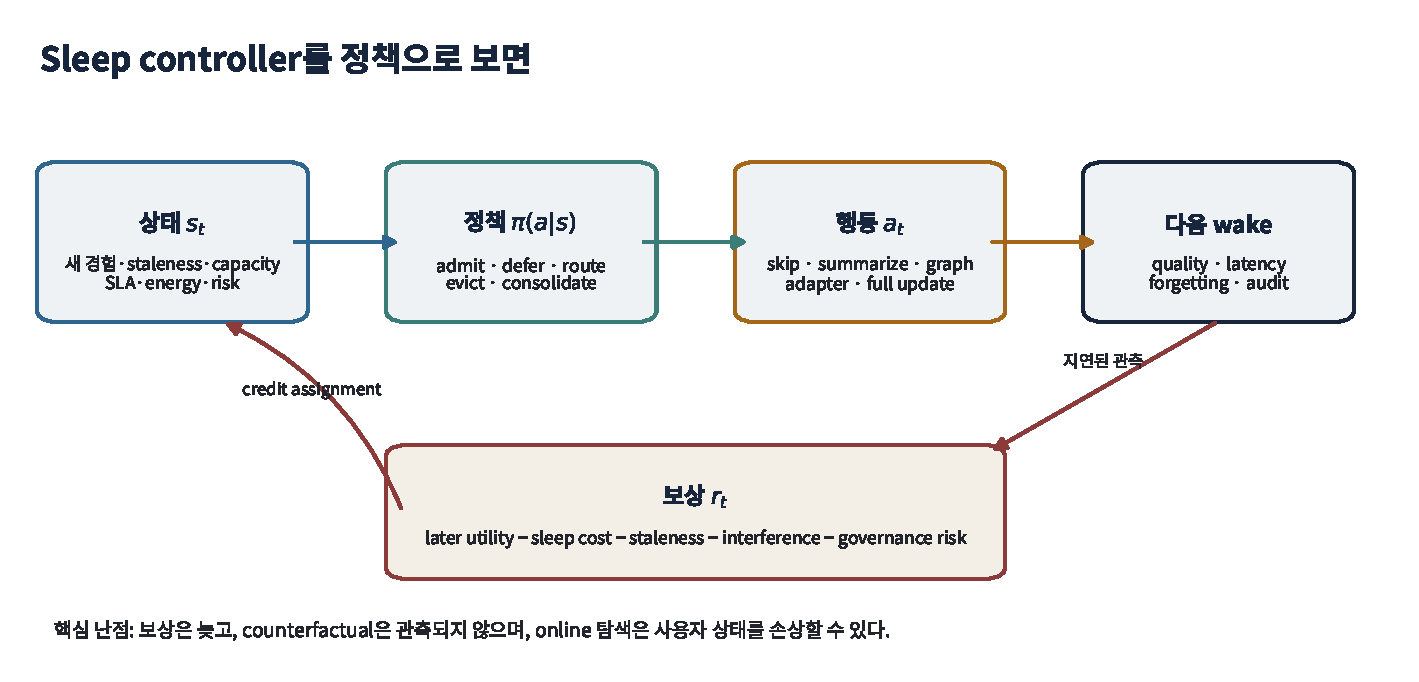
\includegraphics[width=0.94\textwidth]{figures/rl-sleep-policy.pdf}
  \caption{Sleep controller의 강화학습 loop. 실제 보상은 다음 wake period의 utility·forgetting·비용에서
  지연되어 관찰되므로 artifact lineage와 안전한 off-policy evaluation이 필요하다.}
  \figsource{Original synthesis; SRC-STC-0051, SRC-STC-0021}{시스템 상태가 정책으로 들어가고 sleep 행동이 실행된 뒤 다음 wake 결과와 지연 보상이 다시 정책 학습으로 돌아오는 순환도.}
  \label{fig:bg-rl-sleep-policy}
\end{figure}

\section{Offline evaluation이 어려운 이유}

\concept{off-policy-evaluation}{오프폴리시 평가}는 후보 policy를 실제 배포하지 않고 기존 log로
평가한다. 행동 policy $\mu$가 만든 trajectory를 target policy $\pi$에 재가중하는 importance sampling의
기본 형태는

\begin{equation}
\hat V(\pi)=\frac{1}{N}\sum_{i=1}^{N}
\left(\prod_t\frac{\pi(a_t^i|s_t^i)}{\mu(a_t^i|s_t^i)}\right)G_i
\end{equation}

지만 긴 horizon에서는 weight variance가 폭발하고, $\mu(a|s)=0$인 action은 평가할 수 없다. Sleep
action의 downstream utility는 delayed하고 user query가 sparse하므로 model-based simulator와 doubly
robust estimator를 쓰더라도 uncertainty interval을 보고해야 한다.

\begin{table}[htbp]
\centering
\caption{Memory-policy reward를 설계할 때 분리할 signal}
\label{tab:bg-memory-policy-reward}
\small
\begin{tabularx}{\textwidth}{p{0.19\textwidth} X X}
\toprule
Signal & 관측 예 & 잘못 단독 최적화했을 때 \\
\midrule
utility & task success, correction 감소 & benchmark memorization \\
retention & old slice 성능, calibration & 새 변화에 둔감 \\
latency & TTFT/ITL, retrieval hops & 품질이 낮은 aggressive deletion \\
resource & GPU-hour, HBM/SSD bytes, energy & expensive rare capability 제거 \\
governance & scope leak, delete SLA, provenance & 지나친 보수성 또는 미측정 위험 \\
operability & rollback time, version count & 짧은 기간 metric만 선호 \\
\bottomrule
\end{tabularx}
\end{table}

가장 강한 초기 baseline은 learned RL policy가 아니라 explicit rule + constrained optimizer일 수 있다.
RL은 충분한 trajectory coverage와 stable delayed label이 생긴 뒤, trigger와 budget allocation처럼
counterfactual을 시뮬레이션할 수 있는 좁은 action부터 적용한다.
}{}
\IfFileExists{sections/13-meta-learning-ttt.tex}{\chapter{Meta-learning, fast weights, test-time training}
\label{bg:chapter-meta-ttt}

Pre-training과 post-training은 ``배포 전에 무엇을 배울까''를 주로 다룬다. Test-time training과
sleep-time training은 배포 뒤 상태 변화라는 공통점이 있지만 latency path, data window, validation,
persistence가 다르다. 이를 구분하려면 update의 시간척도와 state lifetime을 함께 본다.

\section{Learning to learn: 초기값과 update rule을 학습한다}

\concept{meta-learning}{메타학습}은 여러 task를 경험하며 새 task에 적은 data와 step으로 잘 적응하는
초기값 또는 학습 규칙을 찾는다. MAML의 대표적 형태는 task $\mathcal{T}_i$마다 내부 update

\begin{equation}
\theta'_i=\theta-\alpha\nabla_\theta
\mathcal{L}_{\mathcal{T}_i}^{train}(\theta)
\end{equation}

를 수행한 뒤, 그 결과의 validation loss로 초기값 $\theta$를 갱신한다
\parencite{finn2017maml}.

\concept{bilevel-optimization}{이중수준 최적화}는 ``inner loop에서 adaptation, outer loop에서 그
adaptation 가능성을 평가''하는 구조다.

\begin{equation}
\min_{\theta}\ \mathbb{E}_{\mathcal{T}}
\left[\mathcal{L}^{val}_{\mathcal{T}}
\left(U(\theta,D^{train}_{\mathcal{T}})\right)\right].
\end{equation}

Sleep system에 적용하면 pre/post-training이 좋은 consolidation initializer와 update rule을 배우고,
각 user/device sleep이 local inner loop를 실행할 수 있다. 다만 meta-training task distribution과 실제
user stream이 다르면 ``빠르게 잘못 적응''할 수 있으므로 outer validation에 scope, forgetting, cost를
포함한다.

\section{Fast weights: 상태의 수명을 설계한다}

\concept{fast-weights}{빠른 가중치}는 base weights보다 자주 갱신하고 쉽게 reset하는 parametric state다.
Attention KV cache, recurrent state처럼 gradient 없이 쓰이는 state와 혼동하지 않는다. 여기서는 learned
update로 바뀌며 forward behavior에 들어가는 adapter, memory MLP, normalization parameter 등을 포함한다.

상태를 lifetime으로 나누면 다음과 같다.

\begin{table}[htbp]
\centering
\caption{배포 후 학습 상태의 시간척도}
\label{tab:bg-state-timescale}
\small
\begin{tabularx}{\textwidth}{p{0.18\textwidth} X X X}
\toprule
상태 & update 시점 & persistence & 실패 시 복구 \\
\midrule
query-local & 한 query 내부 & 즉시 폐기 & query 재실행 \\
session fast state & token/session 중 & session 또는 짧은 TTL & session reset \\
user adapter & session 사이 sleep & versioned 장기 & adapter rollback \\
global delta & 여러 cohort 통합 후 & release 단위 & global canary rollback \\
base weights & 드문 offline release & 장기 기준선 & 이전 model release \\
\bottomrule
\end{tabularx}
\end{table}

상태가 오래 살수록 더 많은 validation, provenance, rollback이 필요하다. 빠른 update가 항상 작은
compute라는 뜻도 아니다. token마다 backward하면 작은 parameter라도 latency와 activation memory가
커질 수 있다.

\section{Test-time training의 정확한 경계}

\concept{test-time-training}{테스트 시점 학습}은 test input 자체 또는 가까운 stream에서 자기지도
objective를 만들고 parameter를 갱신해 distribution shift에 적응한다. 초기 연구는 한 unlabeled test
sample의 self-supervised loss로 prediction 전에 update하는 구성을 보였다
\parencite{sun2020ttt}; entropy minimization으로 normalization state를 조정하는 test-time adaptation도
제안되었다 \parencite{wang2021tent}.

다음 세 가지를 구분한다.

\begin{enumerate}
  \item \textbf{TTT-before-answer}: 현재 answer 전에 update가 끝나므로 latency-critical하고 현재 query에
        직접 이익이 있어야 한다.
  \item \textbf{wake consolidation}: session 중 비동기 또는 짧은 idle gap에 최근 stream을 반영한다.
        다음 query부터 유효하지만 아직 wake resource와 충돌한다.
  \item \textbf{sleep training}: 명시적 deferred window에서 더 넓은 replay, validation, compaction,
        publication을 수행한다. 현재 query latency에서 분리된다.
\end{enumerate}

같은 LoRA update도 첫 번째면 TTT, 세 번째면 sleep-time training이다. 따라서 분류 기준은 optimizer나
architecture가 아니라 critical path와 data horizon, persistence, release boundary다.

\section{Reset, accumulation, leakage}

TTT가 sample마다 reset되면 장기기억이 아니고, stream에 누적되면 continual learning이 된다. 누적형은
order sensitivity, adversarial poisoning, user cross-contamination을 받는다. update scope를 query/session/user/
cohort/global로 tag하고 상위 scope로의 승격은 sleep validation을 거치게 한다.

Test input을 학습에 사용한 뒤 같은 sample에서 score를 측정하면 transductive setting이다. 이것을 일반
held-out generalization과 혼동하지 않는다. 더구나 개인 memory에서는 답을 이미 포함한 tool result로
update한 뒤 동일 query를 재평가하면 retrieval cache와 learning gain을 분리할 수 없다.

\begin{keypoint}[Wake와 sleep은 경쟁하는 이름이 아니다]
Wake/test-time update는 즉시 adaptation을, sleep은 replay·compression·cross-session validation과
long-lived publication을 맡는다. 실제 system은 빠른 state가 evidence를 모으고 sleep이 일부를 외부
장기기억이나 parametric artifact로 승격하는 cascade가 된다.
\end{keypoint}
}{}
\IfFileExists{sections/14-editing-unlearning.tex}{\chapter{Model editing과 unlearning: 좁게 바꾸고 정확히 되돌리기}
\label{bg:chapter-editing-unlearning}

Fine-tuning은 dataset 분포 전체에 맞춰 model behavior를 바꾸지만, 때로는 ``A의 CEO는 B가 아니라
C다''처럼 몇 개 fact만 빨리 수정해야 한다. 반대로 삭제 요청은 특정 data의 영향을 제거해야 한다.
두 문제 모두 update 범위, 부작용, provenance, rollback을 요구하지만 성공 기준은 다르다.

\section{Model editing의 네 평가축}

\concept{model-editing}{모델 편집}은 특정 edit request $e=(x_e,y_e)$를 반영하면서 나머지 behavior를
보존하려는 수정이다. ROME은 transformer MLP의 factual association을 찾아 rank-one update를 적용하고
\parencite{meng2022rome}, MEMIT은 이를 많은 memory edit로 확장했다
\parencite{meng2022memit}. 이들은 ``fact가 한 주소에 완전히 저장된다''는 증명이 아니라, 특정
benchmark와 architecture에서 효과적인 intervention을 보인 방법이다.

평가는 최소 네 축으로 나눈다.

\begin{enumerate}
  \item \textbf{efficacy}: edit prompt에서 새 답을 내는가?
  \item \textbf{paraphrase/generalization}: 표현이 달라도 같은 correction을 쓰는가?
  \item \textbf{specificity}: 비슷하지만 다른 entity·relation은 보존되는가?
  \item \textbf{retention}: unrelated capability와 이전 edit가 유지되는가?
\end{enumerate}

\concept{locality}{국소성}은 세 번째와 네 번째를 포괄한다. 단순하게 edit prompt log-probability만
높이면 model이 주변 사실까지 바꾸거나 같은 token을 과도하게 선호할 수 있다. Sleep batch에는 edit
example뿐 아니라 neighborhood, counterfactual, old capability probe가 필요하다.

\section{많은 edit는 다시 continual learning과 capacity 문제가 된다}

한두 edit는 저랭크 update로 가능해 보여도 수천·수백만 edit를 누적하면 interference가 늘어난다.
같은 subject의 시간별 fact가 충돌하고, 이전 edit가 새 edit에 의해 덮이며, 어느 update를 제거해야 하는지
모호해진다. 매일 editing을 반복하는 시스템은 결국 다음 중 하나를 선택해야 한다.

\begin{itemize}
  \item latest fact만 weights에 남기고 history는 temporal external memory에 둔다.
  \item edit를 versioned adapter에 격리하고 주기적으로 merge/distill한다.
  \item 반복 조회되고 안정적인 fact만 parametric promotion하고 나머지는 retrieval한다.
  \item global knowledge refresh는 큰 offline model release에 맡긴다.
\end{itemize}

즉 editing은 sleep-time compute의 가능한 operator이지만, 무한 append 가능한 장기기억 자체는 아니다.

\section{Unlearning은 delete key보다 강한 요구다}

\concept{unlearning}{머신 언러닝}은 지정 data가 학습에 없었던 counterfactual model에 가까워지도록
그 영향을 제거하는 절차다. Sharded, Isolated, Sliced, Aggregated(SISA) training은 data shard별 model을
분리해 삭제 시 영향받은 부분만 재학습하는 방향을 제시했다 \parencite{bourtoule2021unlearning}.

External memory는 item pointer를 지우기 쉬워도 cache, embedding replica, graph edge, summary,
downstream training dataset까지 삭제가 전파되어야 한다. Parametric memory는 어느 weight가 한 record에
기여했는지 역함수가 없으므로 exact deletion이 훨씬 어렵다. ``답을 더 이상 말하지 않는다''와 ``data
영향이 제거되었다''도 다르다.

\begin{table}[htbp]
\centering
\caption{수정·삭제 destination별 복구 성질}
\label{tab:bg-edit-unlearn}
\small
\begin{tabularx}{\textwidth}{p{0.18\textwidth} X X X}
\toprule
Destination & 수정 단위 & 삭제/롤백 & 잔여 위험 \\
\midrule
raw text/log & record/segment & pointer+replica 삭제 & 파생 summary·dataset \\
vector index & vector+metadata & tombstone+rebuild & cache와 stale replica \\
knowledge graph & node/edge/time interval & edge version rollback & derived edge와 conflict \\
adapter/LoRA & file 또는 rank component & version detach & merged artifact, shared behavior \\
base weights & diffuse parameters & retrain/edit/unlearn & 비국소 영향, 검증 비용 \\
\bottomrule
\end{tabularx}
\end{table}

\section{Provenance graph가 architecture choice를 바꾼다}

권리 만료가 잦거나 user delete SLA가 짧다면 external memory나 isolated adapter의 운영 가치가 커진다.
Stable public knowledge처럼 많은 query가 반복되고 source set이 고정될 때는 global parametric refresh가
유리할 수 있다. 따라서 parametric/external 선택은 accuracy 비교만이 아니라 expected delete frequency,
scope, edit conflict, rollback time을 포함한 lifecycle cost 비교다.

\begin{cautionbox}[Negative answer만으로 unlearning을 증명하지 말 것]
모델이 특정 prompt에 답하지 않도록 fine-tune한 것은 suppression일 수 있다. membership inference,
paraphrase, related representation, downstream model lineage를 포함해 요구 수준을 정의해야 한다. 완전한
counterfactual retraining과 근사 unlearning을 보고서에서 구분한다.
\end{cautionbox}
}{}
\IfFileExists{sections/15-training-systems.tex}{\chapter{Training systems: HBM, 통신, checkpoint, publication}
\label{bg:chapter-training-systems}

Sleep-time compute를 ``남는 GPU에서 background fine-tuning''으로만 보면 실제 병목을 놓친다. Training은
weights 외에 gradients, optimizer states, activations, batches를 동시에 움직이고, 후보 artifact를
검증·복제·배포해야 끝난다. 이 장은 알고리즘을 시스템 자원으로 번역한다.

\section{한 step의 memory accounting}

Parameter 수를 $P$, element byte를 $b_w,b_g,b_o$라 하면 단순한 state lower bound는

\begin{equation}
M_{state}\approx P b_w+P b_g+kP b_o+M_{act}+M_{temp},
\end{equation}

이다. Adam의 moment가 두 개면 $k=2$이고, master weight를 별도 유지하면 한 항이 더해진다. Inference는
gradient와 optimizer state가 없지만 training은 forward activation을 backward까지 보존한다.

\concept{mixed-precision}{혼합 정밀도}는 matrix multiply와 저장 일부를 FP16/BF16/FP8로 낮추고 필요한
accumulation이나 master state는 더 높은 precision에 두어 throughput과 안정성을 trade-off한다
\parencite{micikevicius2018mixed}. ``모든 것을 16-bit''라는 뜻이 아니므로 model state별 dtype을
workbook과 checkpoint manifest에 적는다.

\concept{activation-checkpointing}{활성 체크포인팅}은 모든 intermediate activation을 저장하지 않고
일부 boundary만 보존한 뒤 backward에서 forward 일부를 재계산한다. 깊이 $n$ network의 memory를
sublinear하게 줄이는 대신 추가 compute를 쓰는 trade-off가 제시되었다
\parencite{chen2016checkpointing}. Sleep cluster에 idle FLOPs가 있어도 재계산이 wall-clock deadline과
energy budget을 넘는지 봐야 한다.

\begin{figure}[htbp]
  \centering
  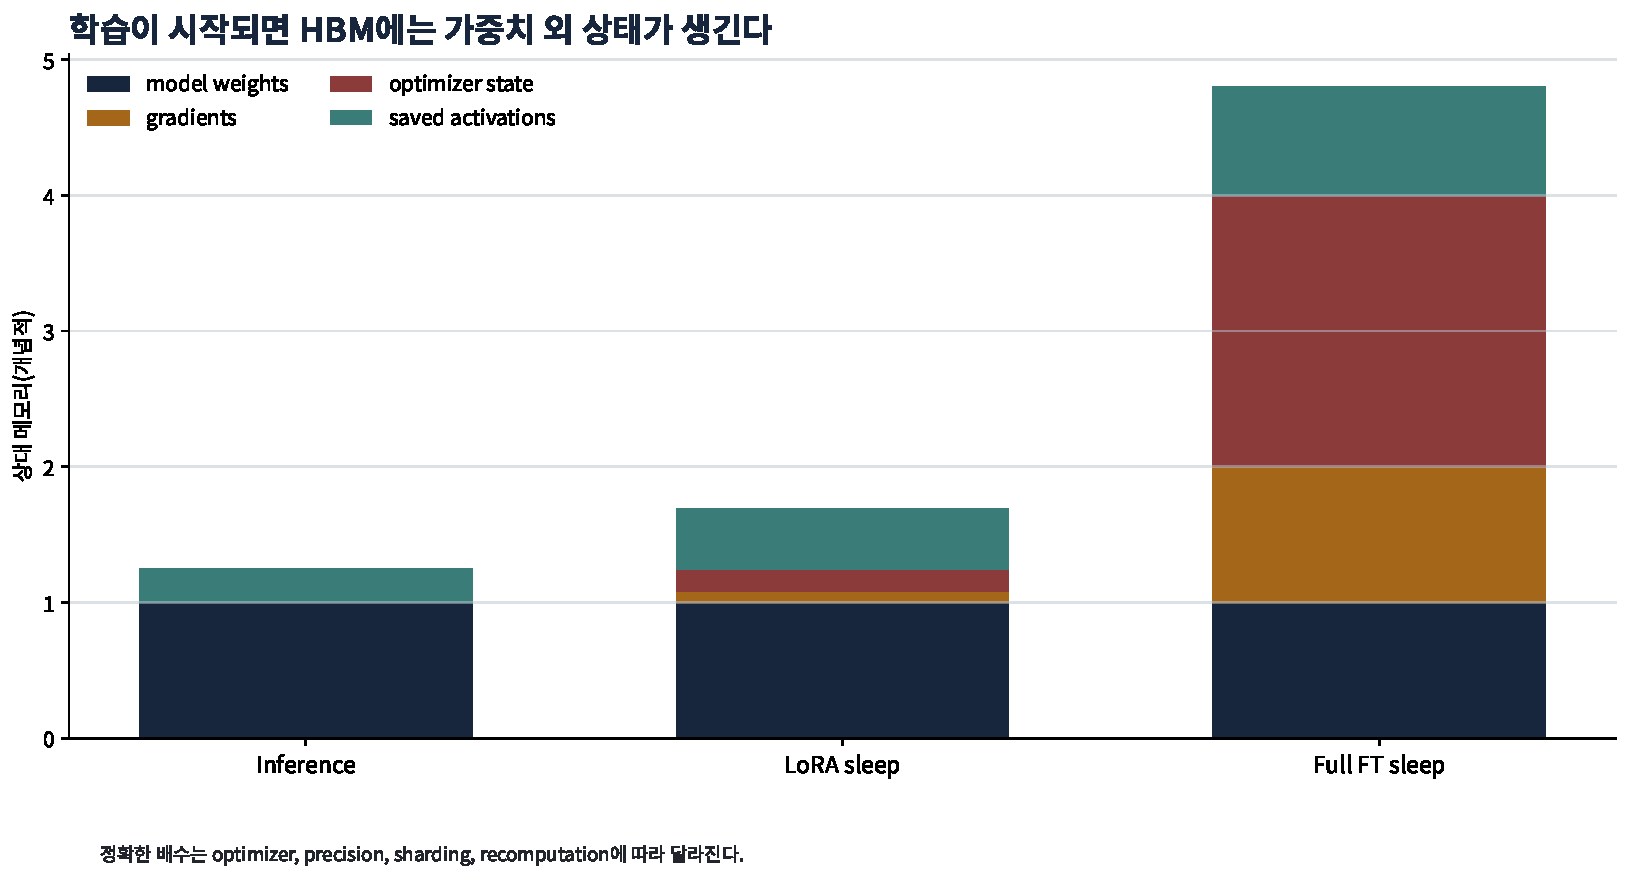
\includegraphics[width=0.94\textwidth]{figures/training-memory-cost.pdf}
  \caption{Inference, LoRA sleep, full fine-tuning sleep의 상대적 state stack. 실제 값은 optimizer,
  precision, sequence, checkpointing, sharding에 따라 달라지므로 이 그림은 구성요소 지도다.}
  \figsource{Original synthesis; SRC-STC-0030, SRC-STC-0021}{세 가지 workload마다 weights, gradients, optimizer state, activations가 층으로 쌓이며 full fine-tuning이 가장 많은 상태를 갖는 비교 그림.}
  \label{fig:bg-training-memory-cost}
\end{figure}

\section{병렬화는 무엇을 복제하고 무엇을 통신하는가}

\concept{data-parallelism}{데이터 병렬화}은 각 device에 model replica를 두고 다른 batch shard를
처리한 뒤 gradient를 all-reduce한다. Compute는 잘 확장하지만 weights와 optimizer state가 복제되고,
짧은 per-user sleep job은 batch가 작아 device utilization이 낮을 수 있다.

\concept{tensor-parallelism}{텐서 병렬화}은 한 layer의 matrix를 여러 device에 나눈다. 큰 model을
fit할 수 있지만 layer마다 collective communication이 발생한다. Megatron-LM은 transformer 내부 model
parallel pattern을 체계화했다 \parencite{shoeybi2019megatron}.

\concept{pipeline-parallelism}{파이프라인 병렬화}은 layer block을 stage로 나누고 microbatch를 흐르게
한다. GPipe는 large model training을 위한 pipeline schedule을 제시했다 \parencite{huang2019gpipe}.
Microbatch가 적으면 stage bubble이 커지므로 작은 sleep job을 개별 pipeline에 넣기보다 여러 tenant job을
privacy boundary 안에서 묶는 scheduler가 필요하다.

\concept{sharding}{샤딩}은 parameter, gradient, optimizer state를 device에 나눠 중복을 줄인다. ZeRO는
data-parallel training의 state redundancy를 단계적으로 제거한다 \parencite{rajbhandari2020zero}.
그러나 shard를 NVMe나 remote memory까지 offload하면 HBM capacity는 줄어도 step마다 read/write traffic과
tail latency가 늘 수 있다.

\begin{table}[htbp]
\centering
\caption{Sleep training job의 주요 data movement}
\label{tab:bg-training-data-movement}
\small
\begin{tabularx}{\textwidth}{p{0.19\textwidth} X X}
\toprule
경로 & 이동하는 상태 & 최적화 질문 \\
\midrule
storage $\rightarrow$ host & replay examples, provenance & sequential batch, compression, filtering locality \\
host $\rightarrow$ HBM & tokens, weights, optimizer shard & pin/prefetch, tenant isolation, reuse \\
GPU $\leftrightarrow$ GPU & activations, gradients, parameters & topology-aware collective, job packing \\
HBM $\leftrightarrow$ NVMe/CXL & cold optimizer, checkpoint, adapter & bandwidth vs recompute, endurance \\
candidate $\rightarrow$ serving & weights/delta/index/graph & atomic publish, cache warmup, rollback copy \\
\bottomrule
\end{tabularx}
\end{table}

\section{Checkpoint가 아니라 release bundle을 version한다}

\concept{versioning}{버전 관리}은 model file 이름만 바꾸는 일이 아니다. 하나의 candidate version은
base model hash, adapter/delta, optimizer continuation state, dataset manifest, code/container, random seed,
hyperparameters, evaluation report, source freeze를 묶는다. 그래야 동일 candidate를 재현하거나 어떤
source가 들어갔는지 판단할 수 있다.

\concept{rollback}{롤백}은 새 artifact pointer를 이전 검증 version으로 원자적으로 전환하고, cache와
replica를 같은 epoch으로 맞추며, 실패 candidate로 만든 후속 data를 quarantine하는 절차다. Rollback
time objective(RTO)와 최대 허용 data loss(RPO)를 external index, adapter, global weights 각각 정의한다.

\concept{publication-gate}{출판 게이트}는 candidate가 offline metric뿐 아니라 retention, privacy scope,
delete compliance, latency, resource budget을 통과할 때만 serving state로 승격하는 boundary다. Training
완료와 publication 완료를 분리하면 실패 후보를 안전하게 분석할 수 있다.

\concept{observability}{관측 가능성}은 sleep job 하나를 event ID에서 serving effect까지 trace할 수 있는
성질이다. 최소 metric은 queue wait, data bytes, H2D/D2H bytes, FLOPs, HBM peak, checkpoint bytes,
validation slices, promotion result, next-wake utility, rollback event다. 평균만이 아니라 tenant와 job size별
tail을 본다.

\section{Memory device 관점의 기회}

Sleep workload는 latency-insensitive하다고 해서 bandwidth-insensitive하지 않다. Full fine-tuning은
optimizer·gradient의 높은-capacity state, replay는 sequential/filtered reads, checkpoint는 large burst
writes, 외부 기억 compaction은 metadata-rich random I/O를 만든다. 따라서 device solution은 다음
primitive를 목표로 할 수 있다.

\begin{itemize}
  \item HBM: active weights, activation, hot optimizer shard의 bandwidth와 capacity,
  \item CXL/host memory: cold optimizer·multi-tenant adapter의 coherent tiering,
  \item NVMe: versioned checkpoint, replay log, index rebuild의 endurance와 predictable QoS,
  \item near-data processing: dedup, compression, vector/graph compaction, checksum/provenance scan,
  \item secure memory: tenant key, erase proof, immutable lineage metadata.
\end{itemize}

기회는 broad parametric sleep이 주류가 되지 않아도 남는다. External-memory consolidation, global model
refresh, checkpointing, index compaction 역시 같은 data movement와 versioning primitive를 사용하기 때문이다.

\begin{keypoint}[Roofline만으로 training job을 설명하지 못한다]
Kernel compute/HBM roofline 외에 interconnect collective, host/storage ingest, checkpoint write, validation
inference, artifact replication을 end-to-end critical path에 넣는다. Sleep window deadline을 넘기면 다음
wake 전에 publication하지 못하므로 throughput이 곧 utility다.
\end{keypoint}
}{}
\IfFileExists{sections/16-stc-mapping.tex}{\chapter{End-to-end mapping: wake 경험에서 검증된 장기기억까지}
\label{bg:chapter-stc-mapping}

앞 장의 용어를 하나의 lifecycle로 조립한다. \concept{wake-state}{Wake 상태}는 사용자 요청을 처리하는
critical path에서 읽히고, query/session 범위에서 빠르게 변할 수 있다. \concept{sleep-state}{Sleep 상태}는
응답 path 밖에서 replay·학습·압축·검증되는 후보다. ``밤''이라는 시각보다 dependency와 latency boundary가
정의의 핵심이다.

\section{두 기억 destination과 hybrid promotion}

\concept{external-memory}{외부 기억}은 text, vector, graph, log처럼 model 밖에서 provenance와 함께
관리되고 query 때 검색된다. \concept{parametric-memory}{모수적 기억}은 base weights, LoRA, adapter,
fast weights처럼 forward 함수 안에서 behavior를 바꾼다.

External memory는 쓰기·삭제·scope·source attribution이 쉽고 capacity를 독립 확장할 수 있지만 retrieval
latency, context token, index drift, tool failure가 있다. Parametric memory는 retrieval 없이 behavior와
skill을 바꿀 수 있지만 update·검증·rollback이 비싸고 exact provenance와 deletion이 어렵다. 따라서
실용적 default는 external system-of-record에 먼저 저장하고, 반복 사용·안정성·scope·break-even이
충분한 pattern만 reversible parametric artifact로 승격하는 hybrid다.

\section{모든 sleep operator를 같은 schema로 기록한다}

\begin{table}[htbp]
\centering
\caption{Sleep operator의 공통 training/serving schema}
\label{tab:bg-stc-operator-schema}
\scriptsize
\begin{tabularx}{\textwidth}{p{0.11\textwidth} p{0.12\textwidth} p{0.12\textwidth} p{0.12\textwidth} X X}
\toprule
Operator & 입력 data & 변경 state & objective/signal & validation & publication/rollback \\
\midrule
summary & episode + source & text record & fidelity+compression & QA, temporal, provenance & record version/tombstone \\
re-embed & text+encoder & vector index & retrieval utility & recall, scope, latency & index epoch/rebuild \\
graph merge & facts+time & node/edge & consistency+coverage & conflict, traversal & edge version/replay log \\
replay FT & new+coreset & LoRA/adapter & task+retention loss & new/old/safety slices & detach previous adapter \\
distill & teacher outputs & student/delta & KL+task loss & fidelity, utility, tail & teacher+student pair \\
model edit & edit+neighbors & localized weights & efficacy+locality & paraphrase, specificity & inverse/version rollback \\
global refresh & curated corpus & base weights & multi-objective & full release suite & model release rollback \\
\bottomrule
\end{tabularx}
\end{table}

각 row는 반드시 teacher/source, trainable state, loss/reward, optimizer, capacity destination, validation,
version을 갖는다. Training kernel이 없는 summary/graph merge도 data transformation objective와 evaluation,
publication이 있으므로 넓은 의미의 sleep compute에 포함된다. 반대로 아무 validation 없이 log를
append하는 것은 consolidation이 아니라 storage다.

\section{Worked example: 반복되는 사용자 correction}

사용자가 여러 session에서 ``회의 요약은 표보다 세 문장 bullet을 선호한다''고 수정했다고 하자.

\begin{enumerate}
  \item \textbf{Wake capture}: correction event와 이전 response, explicit user scope, timestamp를 append한다.
  \item \textbf{Curation}: 일시적 요청인지 stable preference인지 분류하고 중복을 cluster한다.
  \item \textbf{External update}: user profile text/graph에 source-linked preference를 versioned write한다.
  \item \textbf{Benefit measurement}: retrieval이 실제 prompt token과 latency를 얼마나 늘리고, preference가
        얼마나 자주 재사용되는지 관찰한다.
  \item \textbf{Candidate promotion}: 반복 빈도와 stable period가 threshold를 넘으면 user-scoped LoRA
        training set에 positive/negative pair와 general retention replay를 넣는다.
  \item \textbf{Validation}: preference success, unrelated style, safety, other-user non-leakage, latency를 비교한다.
  \item \textbf{Publish}: external profile은 system-of-record로 유지하고 adapter pointer만 canary 승격한다.
  \item \textbf{Evict/rollback}: preference가 바뀌면 old external record를 supersede하고 adapter를 detach 또는
        새 version으로 대체한다.
\end{enumerate}

이 예에서 external과 parametric memory는 경쟁 복제품이 아니다. 하나는 evidence와 control plane,
다른 하나는 반복되는 behavior의 serving accelerator다.

\section{Break-even을 묻는 최소 식}

Parametric promotion의 one-time sleep cost를 $C_{train}+C_{validate}+C_{publish}$, query당 retrieval에서
절약되는 기대 비용을 $\Delta C_{wake}$, 예상 유효 query 수를 $N$, 추가 risk와 maintenance를
$C_{risk}+C_{maint}$라 하면 promotion 조건의 한 baseline은

\begin{equation}
N\,\Delta C_{wake} > C_{train}+C_{validate}+C_{publish}+C_{risk}+C_{maint}.
\end{equation}

정확도/utility gain도 통화 또는 constrained objective로 별도 포함한다. 이 식은 scaling law가 아니라
측정 항목을 빠뜨리지 않기 위한 accounting identity다. $N$을 과대 추정하거나 validation cost를 0으로
두면 대부분의 기억을 weights로 보내는 잘못된 결론이 나온다.

\section{운영 decision tree}

\begin{enumerate}
  \item source와 scope가 불명확하면 학습하지 말고 quarantine한다.
  \item exact delete, temporal history, citation이 중요하면 external system-of-record를 유지한다.
  \item current query만 적응하면 query/session-local state로 제한하고 reset한다.
  \item 반복 사용되는 stable pattern이며 retrieval overhead가 크면 reversible adapter 후보를 만든다.
  \item 여러 사용자에게 일반화되고 독립 evidence가 충분하면 global refresh queue로 승격한다.
  \item 어느 경우든 capacity action과 rollback artifact가 없으면 publish하지 않는다.
\end{enumerate}

\begin{keypoint}[Study Paper를 읽을 때의 질문]
새 sleep-time 연구를 볼 때 ``성능이 올랐나''에 앞서 다음을 확인한다. Wake/sleep 경계는 무엇인가?
무슨 state가 얼마나 오래 바뀌는가? Data source와 replay는 무엇인가? Old capability를 어떻게 평가했는가?
Capacity가 찼을 때 무엇을 지우는가? Candidate는 어떻게 publish·rollback되는가? 이 여섯 질문이 논문
결과를 실제 system과 memory-device workload로 번역한다.
\end{keypoint}
}{}
\IfFileExists{glossary.tex}{\chapter*{용어 사전과 개념 의존성}
\addcontentsline{toc}{chapter}{용어 사전과 개념 의존성}
\markboth{용어 사전과 개념 의존성}{용어 사전과 개념 의존성}
\setcounter{table}{0}
\renewcommand{\thetable}{G.\arabic{table}}
\label{bg:glossary}

이 사전은 Study Paper가 참조하는 canonical concept registry에서 자동 생성한다. 
용어를 단독 정의로만 읽지 말고, 세 번째 열의 prerequisite를 먼저 확인한다. 
본문의 파란 링크는 각 개념이 처음 설명되는 절로 이동한다.

\small
\begin{longtable}{p{0.20\textwidth} p{0.52\textwidth} p{0.18\textwidth}}
\caption{Sleep-time compute를 읽기 위한 canonical glossary}\label{tab:bg-glossary}\\
\toprule
용어 (concept ID) & 한 문장 정의 & 선행 개념 \\
\midrule
\endfirsthead
\toprule
용어 (concept ID) & 한 문장 정의 & 선행 개념 \\
\midrule
\endhead
\midrule\multicolumn{3}{r}{다음 쪽에 계속}\\
\endfoot
\bottomrule
\endlastfoot
\hypertarget{glossary:data}{\hyperref[bg:data]{\textbf{데이터}}} \newline\texttt{data} & 학습이나 평가에 사용되는 관측, 예시, 선호, 경험의 집합이다. & \scriptsize 없음 \\
\hypertarget{glossary:parameter}{\hyperref[bg:parameter]{\textbf{파라미터}}} \newline\texttt{parameter} & 학습으로 값이 바뀌며 모델의 함수를 결정하는 수치다. & \scriptsize 없음 \\
\hypertarget{glossary:forward-pass}{\hyperref[bg:forward-pass]{\textbf{순전파}}} \newline\texttt{forward-pass} & 입력과 현재 파라미터로 예측을 계산하는 과정이다. & \scriptsize data, parameter \\
\hypertarget{glossary:objective}{\hyperref[bg:objective]{\textbf{목적함수}}} \newline\texttt{objective} & 학습이 줄이거나 늘리려는 전체 수치화 목표다. & \scriptsize forward-pass \\
\hypertarget{glossary:loss}{\hyperref[bg:loss]{\textbf{손실}}} \newline\texttt{loss} & 한 예측 또는 배치가 목표와 얼마나 어긋났는지 나타내는 학습 신호다. & \scriptsize objective \\
\hypertarget{glossary:gradient}{\hyperref[bg:gradient]{\textbf{기울기}}} \newline\texttt{gradient} & 각 파라미터를 조금 바꿀 때 손실이 어느 방향으로 얼마나 변하는지 나타낸다. & \scriptsize loss, parameter \\
\hypertarget{glossary:backpropagation}{\hyperref[bg:backpropagation]{\textbf{역전파}}} \newline\texttt{backpropagation} & 출력의 손실에서 각 파라미터의 기울기를 연쇄법칙으로 계산하는 절차다. & \scriptsize forward-pass, gradient \\
\hypertarget{glossary:optimizer}{\hyperref[bg:optimizer]{\textbf{옵티마이저}}} \newline\texttt{optimizer} & 기울기와 내부 상태를 사용해 파라미터를 갱신하는 규칙이다. & \scriptsize gradient \\
\hypertarget{glossary:learning-rate}{\hyperref[bg:learning-rate]{\textbf{학습률}}} \newline\texttt{learning-rate} & 한 갱신에서 기울기를 얼마나 크게 반영할지 정하는 크기다. & \scriptsize optimizer \\
\hypertarget{glossary:optimizer-state}{\hyperref[bg:optimizer-state]{\textbf{옵티마이저 상태}}} \newline\texttt{optimizer-state} & 모멘텀과 분산 추정치처럼 옵티마이저가 파라미터 외에 유지하는 상태다. & \scriptsize optimizer \\
\hypertarget{glossary:batch}{\hyperref[bg:batch]{\textbf{배치}}} \newline\texttt{batch} & 한 번의 갱신을 위해 함께 처리하는 예시 묶음이다. & \scriptsize data, loss \\
\hypertarget{glossary:epoch}{\hyperref[bg:epoch]{\textbf{에폭}}} \newline\texttt{epoch} & 학습 데이터 전체를 대략 한 번 소비한 단위다. & \scriptsize batch \\
\hypertarget{glossary:sampling}{\hyperref[bg:sampling]{\textbf{샘플링}}} \newline\texttt{sampling} & 전체 데이터에서 다음 학습 예시나 배치를 선택하는 규칙이다. & \scriptsize data, batch \\
\hypertarget{glossary:validation-set}{\hyperref[bg:validation-set]{\textbf{검증 세트}}} \newline\texttt{validation-set} & 학습에는 직접 쓰지 않고 설정 선택과 조기 종료에 사용하는 데이터다. & \scriptsize data \\
\hypertarget{glossary:test-set}{\hyperref[bg:test-set]{\textbf{테스트 세트}}} \newline\texttt{test-set} & 최종 선택 뒤 일반화 성능을 추정하기 위해 보존하는 데이터다. & \scriptsize validation-set \\
\hypertarget{glossary:overfitting}{\hyperref[bg:overfitting]{\textbf{과적합}}} \newline\texttt{overfitting} & 학습 데이터에는 잘 맞지만 새로운 데이터에는 성능이 낮아지는 현상이다. & \scriptsize validation-set \\
\hypertarget{glossary:generalization}{\hyperref[bg:generalization]{\textbf{일반화}}} \newline\texttt{generalization} & 학습에서 보지 못한 입력에서도 유용한 성능을 유지하는 능력이다. & \scriptsize test-set, overfitting \\
\hypertarget{glossary:pretraining}{\hyperref[bg:pretraining]{\textbf{사전학습}}} \newline\texttt{pretraining} & 배포 전 대규모 데이터로 범용 모델을 처음 형성하는 학습이다. & \scriptsize objective, batch \\
\hypertarget{glossary:continued-pretraining}{\hyperref[bg:continued-pretraining]{\textbf{지속 사전학습}}} \newline\texttt{continued-pretraining} & 기존 사전학습 모델을 추가 비지도 또는 자기지도 코퍼스로 계속 학습하는 방식이다. & \scriptsize pretraining \\
\hypertarget{glossary:fine-tuning}{\hyperref[bg:fine-tuning]{\textbf{미세조정}}} \newline\texttt{fine-tuning} & 사전학습 모델을 더 좁은 데이터와 목적에 맞게 추가 학습하는 방식이다. & \scriptsize pretraining \\
\hypertarget{glossary:instruction-tuning}{\hyperref[bg:instruction-tuning]{\textbf{지시 튜닝}}} \newline\texttt{instruction-tuning} & 지시와 응답 쌍으로 지시 따르기 행동을 학습하는 미세조정이다. & \scriptsize fine-tuning, supervision \\
\hypertarget{glossary:preference-optimization}{\hyperref[bg:preference-optimization]{\textbf{선호 최적화}}} \newline\texttt{preference-optimization} & 사람 또는 모델이 선호한 출력 쪽으로 정책을 이동시키는 후학습 계열이다. & \scriptsize fine-tuning, loss \\
\hypertarget{glossary:supervision}{\hyperref[bg:supervision]{\textbf{지도 신호}}} \newline\texttt{supervision} & 입력에 대해 원하는 목표나 비교 신호를 외부에서 제공하는 학습 방식이다. & \scriptsize data, loss \\
\hypertarget{glossary:self-supervision}{\hyperref[bg:self-supervision]{\textbf{자기지도학습}}} \newline\texttt{self-supervision} & 원시 데이터 자체에서 마스킹이나 다음 토큰 같은 목표를 구성하는 학습 방식이다. & \scriptsize supervision \\
\hypertarget{glossary:representation}{\hyperref[bg:representation]{\textbf{표현}}} \newline\texttt{representation} & 모델이 입력의 정보를 후속 계산에 쓰기 좋은 내부 벡터나 상태로 표현한 것이다. & \scriptsize forward-pass \\
\hypertarget{glossary:logit}{\hyperref[bg:logit]{\textbf{로짓}}} \newline\texttt{logit} & 확률 정규화 전 모델이 각 선택지에 부여한 점수다. & \scriptsize forward-pass \\
\hypertarget{glossary:softmax}{\hyperref[bg:softmax]{\textbf{소프트맥스}}} \newline\texttt{softmax} & 로짓을 합이 1인 확률 분포로 바꾸는 함수다. & \scriptsize logit \\
\hypertarget{glossary:cross-entropy}{\hyperref[bg:cross-entropy]{\textbf{교차엔트로피}}} \newline\texttt{cross-entropy} & 목표 분포에 높은 확률을 주도록 만드는 대표적 분류·언어모델 손실이다. & \scriptsize softmax, loss \\
\hypertarget{glossary:distillation}{\hyperref[bg:distillation]{\textbf{지식 증류}}} \newline\texttt{distillation} & 교사 모델의 출력이나 내부 신호를 학생 모델이 모방하도록 학습하는 방식이다. & \scriptsize loss, softmax \\
\hypertarget{glossary:teacher-model}{\hyperref[bg:teacher-model]{\textbf{교사 모델}}} \newline\texttt{teacher-model} & 증류 목표를 제공하는 기준 모델 또는 모델 집합이다. & \scriptsize distillation \\
\hypertarget{glossary:student-model}{\hyperref[bg:student-model]{\textbf{학생 모델}}} \newline\texttt{student-model} & 교사의 행동이나 분포를 학습하는 대상 모델이다. & \scriptsize distillation \\
\hypertarget{glossary:kl-divergence}{\hyperref[bg:kl-divergence]{\textbf{KL 발산}}} \newline\texttt{kl-divergence} & 두 확률 분포의 불일치를 한 방향으로 측정하는 양이다. & \scriptsize softmax \\
\hypertarget{glossary:temperature}{\hyperref[bg:temperature]{\textbf{온도}}} \newline\texttt{temperature} & 확률 분포의 날카로움과 탐색 정도를 조절하는 스케일이다. & \scriptsize softmax \\
\hypertarget{glossary:peft}{\hyperref[bg:peft]{\textbf{PEFT}}} \newline\texttt{peft} & 전체 가중치 대신 작은 일부 상태만 학습하는 파라미터 효율 미세조정이다. & \scriptsize fine-tuning, parameter \\
\hypertarget{glossary:lora}{\hyperref[bg:lora]{\textbf{LoRA}}} \newline\texttt{lora} & 가중치 변화량을 두 저랭크 행렬의 곱으로 제한하는 PEFT 방식이다. & \scriptsize peft \\
\hypertarget{glossary:adapter}{\hyperref[bg:adapter]{\textbf{어댑터}}} \newline\texttt{adapter} & 기본 모델 사이에 삽입하거나 별도로 결합하는 작은 학습 모듈이다. & \scriptsize peft \\
\hypertarget{glossary:mixture-of-experts}{\hyperref[bg:mixture-of-experts]{\textbf{MoE}}} \newline\texttt{mixture-of-experts} & 입력마다 일부 전문가 모듈만 선택해 계산하는 희소 모델 구조다. & \scriptsize parameter, forward-pass \\
\hypertarget{glossary:trainable-state}{\hyperref[bg:trainable-state]{\textbf{학습 가능 상태}}} \newline\texttt{trainable-state} & 한 학습 단계에서 실제로 갱신 가능한 파라미터와 보조 상태의 집합이다. & \scriptsize parameter, optimizer-state \\
\hypertarget{glossary:serving-artifact}{\hyperref[bg:serving-artifact]{\textbf{서빙 산출물}}} \newline\texttt{serving-artifact} & 학습이 끝난 뒤 추론에 배포되는 가중치, 어댑터, 인덱스 또는 그래프다. & \scriptsize trainable-state \\
\hypertarget{glossary:data-curation}{\hyperref[bg:data-curation]{\textbf{데이터 큐레이션}}} \newline\texttt{data-curation} & 목표와 정책에 맞는 학습 후보를 수집·정규화·중복 제거·분류하는 과정이다. & \scriptsize data \\
\hypertarget{glossary:data-filtering}{\hyperref[bg:data-filtering]{\textbf{데이터 필터링}}} \newline\texttt{data-filtering} & 품질·안전·권리·관련성 기준으로 학습 후보를 남기거나 제외하는 절차다. & \scriptsize data-curation \\
\hypertarget{glossary:data-augmentation}{\hyperref[bg:data-augmentation]{\textbf{데이터 증강}}} \newline\texttt{data-augmentation} & 의미상 보존하려는 속성을 유지하면서 학습 예시의 변형을 만드는 방법이다. & \scriptsize data \\
\hypertarget{glossary:synthetic-data}{\hyperref[bg:synthetic-data]{\textbf{합성 데이터}}} \newline\texttt{synthetic-data} & 모델·규칙·시뮬레이터가 생성한 학습 또는 평가 예시다. & \scriptsize data \\
\hypertarget{glossary:provenance}{\hyperref[bg:provenance]{\textbf{출처 추적성}}} \newline\texttt{provenance} & 데이터와 산출물이 어디서 왔고 어떤 변환·검증을 거쳤는지 추적하는 기록이다. & \scriptsize data \\
\hypertarget{glossary:replay-buffer}{\hyperref[bg:replay-buffer]{\textbf{리플레이 버퍼}}} \newline\texttt{replay-buffer} & 미래 학습에서 다시 사용할 과거 경험이나 예시를 제한된 용량으로 보관한 저장소다. & \scriptsize sampling, data \\
\hypertarget{glossary:coreset}{\hyperref[bg:coreset]{\textbf{코어셋}}} \newline\texttt{coreset} & 전체 과거 데이터를 대표하도록 선택한 작은 가중 표본 집합이다. & \scriptsize replay-buffer \\
\hypertarget{glossary:generated-replay}{\hyperref[bg:generated-replay]{\textbf{생성 리플레이}}} \newline\texttt{generated-replay} & 원본 예시 대신 생성 모델이 복원한 과거 분포의 표본을 재학습에 쓰는 방식이다. & \scriptsize synthetic-data, replay-buffer \\
\hypertarget{glossary:continual-learning}{\hyperref[bg:continual-learning]{\textbf{지속학습}}} \newline\texttt{continual-learning} & 시간에 따라 도착하는 데이터나 과제를 배우면서 이전 능력을 유지하는 학습 설정이다. & \scriptsize fine-tuning \\
\hypertarget{glossary:catastrophic-forgetting}{\hyperref[bg:catastrophic-forgetting]{\textbf{파국적 망각}}} \newline\texttt{catastrophic-forgetting} & 새 학습 뒤 이전 데이터나 과제 성능이 급격히 무너지는 현상이다. & \scriptsize continual-learning \\
\hypertarget{glossary:stability-plasticity}{\hyperref[bg:stability-plasticity]{\textbf{안정성–가소성}}} \newline\texttt{stability-plasticity} & 기존 능력을 안정적으로 보존하는 힘과 새 정보를 빠르게 배우는 가소성 사이의 긴장이다. & \scriptsize continual-learning \\
\hypertarget{glossary:backward-transfer}{\hyperref[bg:backward-transfer]{\textbf{후방 전이}}} \newline\texttt{backward-transfer} & 새 학습이 과거 과제 성능을 높이거나 낮추는 효과다. & \scriptsize continual-learning \\
\hypertarget{glossary:regularization}{\hyperref[bg:regularization]{\textbf{정규화}}} \newline\texttt{regularization} & 원하는 해의 성질이나 과거 상태 보존을 손실에 제약으로 더하는 방법이다. & \scriptsize loss \\
\hypertarget{glossary:ewc}{\hyperref[bg:ewc]{\textbf{EWC}}} \newline\texttt{ewc} & 과거 과제에 중요했던 가중치의 이동을 중요도에 비례해 벌점 주는 지속학습 방법이다. & \scriptsize regularization, catastrophic-forgetting \\
\hypertarget{glossary:gradient-projection}{\hyperref[bg:gradient-projection]{\textbf{기울기 투영}}} \newline\texttt{gradient-projection} & 새 기울기를 허용된 제약 영역으로 투영해 과거 손실의 악화를 제한하는 방법이다. & \scriptsize gradient \\
\hypertarget{glossary:gem}{\hyperref[bg:gem]{\textbf{GEM}}} \newline\texttt{gem} & episodic memory의 과거 기울기를 제약으로 사용하는 Gradient Episodic Memory 방법이다. & \scriptsize gradient-projection, replay-buffer \\
\hypertarget{glossary:parameter-isolation}{\hyperref[bg:parameter-isolation]{\textbf{파라미터 격리}}} \newline\texttt{parameter-isolation} & 과제·사용자·시기별로 다른 파라미터 부분을 배정해 간섭을 막는 방법이다. & \scriptsize parameter, continual-learning \\
\hypertarget{glossary:dynamic-expansion}{\hyperref[bg:dynamic-expansion]{\textbf{동적 확장}}} \newline\texttt{dynamic-expansion} & 기존 용량이 부족할 때 모듈이나 파라미터를 동적으로 추가하는 방법이다. & \scriptsize parameter-isolation \\
\hypertarget{glossary:pruning}{\hyperref[bg:pruning]{\textbf{프루닝}}} \newline\texttt{pruning} & 중요도가 낮은 연결·모듈·기억을 제거해 용량과 계산을 회수하는 과정이다. & \scriptsize parameter \\
\hypertarget{glossary:capacity-budget}{\hyperref[bg:capacity-budget]{\textbf{용량 예산}}} \newline\texttt{capacity-budget} & 정확도·지연·비용·권리 제약 아래 한 계층이 사용할 수 있는 저장·상태 한도다. & \scriptsize serving-artifact \\
\hypertarget{glossary:compression}{\hyperref[bg:compression]{\textbf{압축}}} \newline\texttt{compression} & 허용 가능한 정보 손실 아래 상태나 데이터를 더 작은 표현으로 바꾸는 과정이다. & \scriptsize capacity-budget \\
\hypertarget{glossary:rate-distortion}{\hyperref[bg:rate-distortion]{\textbf{율–왜곡}}} \newline\texttt{rate-distortion} & 표현률 또는 저장 비용과 허용 왜곡 사이의 최적 trade-off를 다루는 관점이다. & \scriptsize compression, loss \\
\hypertarget{glossary:memory-admission}{\hyperref[bg:memory-admission]{\textbf{기억 입장 정책}}} \newline\texttt{memory-admission} & 새 경험을 어느 기억 계층에 넣을지 또는 버릴지 결정하는 정책이다. & \scriptsize capacity-budget \\
\hypertarget{glossary:memory-eviction}{\hyperref[bg:memory-eviction]{\textbf{기억 퇴거 정책}}} \newline\texttt{memory-eviction} & 용량을 회수하기 위해 어떤 기존 기억을 제거·축약·하향 이동할지 정하는 정책이다. & \scriptsize memory-admission \\
\hypertarget{glossary:consolidation}{\hyperref[bg:consolidation]{\textbf{공고화}}} \newline\texttt{consolidation} & 여러 경험을 재생·요약·결합해 더 안정적이고 장기적인 상태로 전환하는 과정이다. & \scriptsize continual-learning, replay-buffer \\
\hypertarget{glossary:rl-state}{\hyperref[bg:rl-state]{\textbf{RL 상태}}} \newline\texttt{rl-state} & 의사결정 시점에 정책이 관측하는 환경·시스템·기억의 정보다. & \scriptsize data \\
\hypertarget{glossary:action}{\hyperref[bg:action]{\textbf{행동}}} \newline\texttt{action} & 정책이 상태를 보고 선택해 환경이나 기억 시스템을 바꾸는 조작이다. & \scriptsize rl-state \\
\hypertarget{glossary:reward}{\hyperref[bg:reward]{\textbf{보상}}} \newline\texttt{reward} & 행동 결과의 바람직함을 수치로 제공하는 학습 신호다. & \scriptsize action \\
\hypertarget{glossary:trajectory}{\hyperref[bg:trajectory]{\textbf{궤적}}} \newline\texttt{trajectory} & 시간 순서로 이어진 상태·행동·보상의 열이다. & \scriptsize rl-state, action, reward \\
\hypertarget{glossary:return}{\hyperref[bg:return]{\textbf{리턴}}} \newline\texttt{return} & 현재 이후 보상을 할인해 더한 누적 성과다. & \scriptsize trajectory \\
\hypertarget{glossary:policy}{\hyperref[bg:policy]{\textbf{정책}}} \newline\texttt{policy} & 상태에서 행동의 확률 또는 선택으로 가는 의사결정 규칙이다. & \scriptsize rl-state, action \\
\hypertarget{glossary:value-function}{\hyperref[bg:value-function]{\textbf{가치 함수}}} \newline\texttt{value-function} & 한 상태나 상태–행동에서 기대되는 미래 return을 추정하는 함수다. & \scriptsize return, rl-state \\
\hypertarget{glossary:credit-assignment}{\hyperref[bg:credit-assignment]{\textbf{신용 할당}}} \newline\texttt{credit-assignment} & 지연된 결과의 책임이나 공을 과거 행동과 상태에 배분하는 문제다. & \scriptsize return, action \\
\hypertarget{glossary:policy-gradient}{\hyperref[bg:policy-gradient]{\textbf{정책 기울기}}} \newline\texttt{policy-gradient} & 기대 return이 증가하도록 정책 파라미터의 기울기를 추정하는 방법이다. & \scriptsize policy, gradient, return \\
\hypertarget{glossary:on-policy}{\hyperref[bg:on-policy]{\textbf{온폴리시}}} \newline\texttt{on-policy} & 현재 학습 중인 정책이 수집한 경험으로 그 정책을 갱신하는 설정이다. & \scriptsize policy \\
\hypertarget{glossary:off-policy}{\hyperref[bg:off-policy]{\textbf{오프폴리시}}} \newline\texttt{off-policy} & 현재 정책과 다른 과거·행동 정책이 수집한 경험도 학습에 사용하는 설정이다. & \scriptsize policy, replay-buffer \\
\hypertarget{glossary:reward-model}{\hyperref[bg:reward-model]{\textbf{보상 모델}}} \newline\texttt{reward-model} & 사람이나 모델의 비교 선호에서 출력의 품질 점수를 근사한 모델이다. & \scriptsize preference-optimization \\
\hypertarget{glossary:rlhf}{\hyperref[bg:rlhf]{\textbf{RLHF}}} \newline\texttt{rlhf} & 사람 피드백으로 학습한 보상이나 선호를 이용해 모델 정책을 조정하는 절차다. & \scriptsize reward-model, policy-gradient \\
\hypertarget{glossary:rlaif}{\hyperref[bg:rlaif]{\textbf{RLAIF}}} \newline\texttt{rlaif} & 사람 대신 또는 사람과 함께 AI가 만든 피드백을 이용하는 선호 학습 절차다. & \scriptsize rlhf \\
\hypertarget{glossary:dpo}{\hyperref[bg:dpo]{\textbf{DPO}}} \newline\texttt{dpo} & 명시적 보상 모델과 online RL rollout 없이 선호 쌍으로 정책을 직접 최적화하는 방법이다. & \scriptsize preference-optimization \\
\hypertarget{glossary:off-policy-evaluation}{\hyperref[bg:off-policy-evaluation]{\textbf{오프폴리시 평가}}} \newline\texttt{off-policy-evaluation} & 새 정책을 실제 배포하지 않고 과거 로그로 기대 성과를 추정하는 평가다. & \scriptsize off-policy, validation-set \\
\hypertarget{glossary:meta-learning}{\hyperref[bg:meta-learning]{\textbf{메타학습}}} \newline\texttt{meta-learning} & 새 과제나 데이터에 적은 단계로 잘 적응하도록 학습 절차 자체를 학습하는 관점이다. & \scriptsize fine-tuning \\
\hypertarget{glossary:bilevel-optimization}{\hyperref[bg:bilevel-optimization]{\textbf{이중수준 최적화}}} \newline\texttt{bilevel-optimization} & 내부 적응 결과를 바깥 목표로 평가해 초기값이나 학습 규칙을 최적화하는 중첩 문제다. & \scriptsize meta-learning, objective \\
\hypertarget{glossary:fast-weights}{\hyperref[bg:fast-weights]{\textbf{빠른 가중치}}} \newline\texttt{fast-weights} & base weights보다 빠르게, 짧은 범위에서 갱신·폐기되는 파라미터성 상태다. & \scriptsize parameter \\
\hypertarget{glossary:test-time-training}{\hyperref[bg:test-time-training]{\textbf{테스트 시점 학습}}} \newline\texttt{test-time-training} & 배포 후 현재 또는 최근 입력에서 만든 목표로 추론 경로 안팎에서 상태를 갱신하는 학습이다. & \scriptsize fast-weights, self-supervision \\
\hypertarget{glossary:model-editing}{\hyperref[bg:model-editing]{\textbf{모델 편집}}} \newline\texttt{model-editing} & 좁은 사실이나 행동을 국소적으로 바꾸면서 나머지 능력을 보존하려는 모델 수정이다. & \scriptsize parameter \\
\hypertarget{glossary:locality}{\hyperref[bg:locality]{\textbf{국소성}}} \newline\texttt{locality} & 의도한 대상 밖의 예측과 능력이 수정 전과 가깝게 유지되는 성질이다. & \scriptsize model-editing, generalization \\
\hypertarget{glossary:unlearning}{\hyperref[bg:unlearning]{\textbf{머신 언러닝}}} \newline\texttt{unlearning} & 지정 데이터나 그 영향이 학습되지 않은 상태에 가깝도록 제거하는 절차다. & \scriptsize model-editing, provenance \\
\hypertarget{glossary:mixed-precision}{\hyperref[bg:mixed-precision]{\textbf{혼합 정밀도}}} \newline\texttt{mixed-precision} & 정확도와 안정성을 지키며 연산·상태별로 서로 다른 수치 정밀도를 쓰는 학습 기법이다. & \scriptsize trainable-state \\
\hypertarget{glossary:activation-checkpointing}{\hyperref[bg:activation-checkpointing]{\textbf{활성 체크포인팅}}} \newline\texttt{activation-checkpointing} & 일부 activation만 저장하고 backward 때 나머지를 재계산해 메모리를 절약하는 기법이다. & \scriptsize forward-pass \\
\hypertarget{glossary:data-parallelism}{\hyperref[bg:data-parallelism]{\textbf{데이터 병렬화}}} \newline\texttt{data-parallelism} & 장치마다 다른 batch shard를 처리하고 gradient를 결합하는 병렬화다. & \scriptsize batch \\
\hypertarget{glossary:tensor-parallelism}{\hyperref[bg:tensor-parallelism]{\textbf{텐서 병렬화}}} \newline\texttt{tensor-parallelism} & 한 층의 텐서 연산과 파라미터를 여러 장치에 나누는 병렬화다. & \scriptsize parameter \\
\hypertarget{glossary:pipeline-parallelism}{\hyperref[bg:pipeline-parallelism]{\textbf{파이프라인 병렬화}}} \newline\texttt{pipeline-parallelism} & 연속된 층 구간을 여러 stage에 배치하고 microbatch를 파이프라인으로 흘리는 병렬화다. & \scriptsize forward-pass \\
\hypertarget{glossary:sharding}{\hyperref[bg:sharding]{\textbf{샤딩}}} \newline\texttt{sharding} & 파라미터·gradient·optimizer state를 장치나 저장 계층에 분할 배치하는 방법이다. & \scriptsize optimizer-state, parameter \\
\hypertarget{glossary:versioning}{\hyperref[bg:versioning]{\textbf{버전 관리}}} \newline\texttt{versioning} & 학습 데이터·코드·상태·평가·산출물을 함께 식별 가능한 버전으로 묶는 관리다. & \scriptsize serving-artifact \\
\hypertarget{glossary:rollback}{\hyperref[bg:rollback]{\textbf{롤백}}} \newline\texttt{rollback} & 실패한 새 상태를 중단하고 검증된 이전 상태로 원자적으로 되돌리는 절차다. & \scriptsize versioning \\
\hypertarget{glossary:publication-gate}{\hyperref[bg:publication-gate]{\textbf{출판 게이트}}} \newline\texttt{publication-gate} & 후보 상태가 검증·안전·권리·비용 기준을 통과할 때만 serving에 승격하는 경계다. & \scriptsize validation-set, versioning \\
\hypertarget{glossary:wake-state}{\hyperref[bg:wake-state]{\textbf{Wake 상태}}} \newline\texttt{wake-state} & 사용자 요청을 처리하는 latency-critical 경로에서 읽거나 짧게 갱신되는 상태다. & \scriptsize serving-artifact \\
\hypertarget{glossary:sleep-state}{\hyperref[bg:sleep-state]{\textbf{Sleep 상태}}} \newline\texttt{sleep-state} & 응답 경로 밖에서 재생·압축·학습·검증·승격되는 deferred 상태다. & \scriptsize wake-state, continual-learning \\
\hypertarget{glossary:parametric-memory}{\hyperref[bg:parametric-memory]{\textbf{모수적 기억}}} \newline\texttt{parametric-memory} & 모델 가중치·어댑터·fast weights처럼 forward 함수 안에 내재된 기억 상태다. & \scriptsize parameter \\
\hypertarget{glossary:external-memory}{\hyperref[bg:external-memory]{\textbf{외부 기억}}} \newline\texttt{external-memory} & text·vector·graph·log처럼 모델 밖에 저장되어 검색과 도구 호출로 사용되는 기억이다. & \scriptsize data \\
\hypertarget{glossary:memory-routing}{\hyperref[bg:memory-routing]{\textbf{기억 라우팅}}} \newline\texttt{memory-routing} & 질의와 상태에 따라 외부 기억·fast state·parametric state 중 어디를 읽고 쓸지 정하는 제어다. & \scriptsize external-memory, parametric-memory \\
\hypertarget{glossary:observability}{\hyperref[bg:observability]{\textbf{관측 가능성}}} \newline\texttt{observability} & 데이터·학습·평가·배포 상태와 실패 원인을 지표·로그·trace로 재구성할 수 있는 성질이다. & \scriptsize publication-gate \\
\end{longtable}
\normalsize

\begin{keypoint}[의존성 표를 사용하는 법]
어떤 Study claim이 낯설다면 해당 concept ID의 본문 label로 이동하고, 선행 개념을 
왼쪽에서 오른쪽 순서로 읽는다. 용어 정의는 결과를 보장하지 않는다. 예를 들어 
\texttt{unlearning}의 정의를 안다는 것은 특정 방법이 삭제 요구를 완전히 충족한다는 뜻이 아니다.
\end{keypoint}
}{}

\backmatter
\printbibliography[heading=bibintoc,title={참고문헌}]
\end{document}
